% Capitolul 3: Modele VAR structurale și proiecții locale
% Analiza avansată a seriilor de timp și previziune -- Programul de master Statistică aplicată și data science, anul I, semestrul 2, Academia de Studii Economice din București
% GENERAT de latex/build_chapter3.py -- modificați generatorul, nu acest fișier.

\newcommand{\coursename}{Analiza avansată a seriilor de timp și previziune}
\def\atslang{ro}
% Preambul comun ATS -- Analiza avansată a seriilor de timp și previziune / Advanced Time Series Analysis and Forecasting
% (Beamer, 16:9). Același design ca MFM, SFM și TSA (copiat din TSA, 5 octombrie 2026). Înainte de % Preambul comun ATS -- Analiza avansată a seriilor de timp și previziune / Advanced Time Series Analysis and Forecasting
% (Beamer, 16:9). Același design ca MFM, SFM și TSA (copiat din TSA, 5 octombrie 2026). Înainte de % Preambul comun ATS -- Analiza avansată a seriilor de timp și previziune / Advanced Time Series Analysis and Forecasting
% (Beamer, 16:9). Același design ca MFM, SFM și TSA (copiat din TSA, 5 octombrie 2026). Înainte de \input{../../latex/preamble} se definește
%   \newcommand{\coursename}{Advanced Time Series Analysis and Forecasting}          (EN)
%   \newcommand{\coursename}{Analiza avansată a seriilor de timp și previziune}       (RO)  și  \def\atslang{ro}
% Fișierele .tex se află în EN/Courses, EN/Seminars, RO/Cursuri, RO/Seminarii (două niveluri sub rădăcină).
% Deck-urile sînt generate de latex/build_chapterN.py / build_seminarN.py (vezi latex/ats_build.py).

\documentclass[9pt, aspectratio=169, t]{beamer}
\providecommand{\coursename}{Advanced Time Series Analysis and Forecasting}

% Ensure content fits on slides
\setbeamersize{text margin left=8mm, text margin right=8mm}
% Smaller institute font (title page)
\setbeamerfont{institute}{size=\footnotesize}

%=============================================================================
% THEME AND STYLE CONFIGURATION
%=============================================================================
\usetheme{default}
% Using default theme for clean header/footer control

% Color Palette (matching Redispatch PDF)
\definecolor{MainBlue}{RGB}{26, 58, 110}
\definecolor{AccentBlue}{RGB}{26, 58, 110}
\definecolor{IDAred}{RGB}{205, 0, 0}
\definecolor{DarkGray}{RGB}{51, 51, 51}
\definecolor{MediumGray}{RGB}{128, 128, 128}
\definecolor{LightGray}{RGB}{248, 248, 248}
\definecolor{VeryLightGray}{RGB}{235, 235, 235}
\definecolor{KeynoteGray}{RGB}{218, 218, 218}
\definecolor{SectionGray}{RGB}{120, 120, 120}
\definecolor{FooterGray}{RGB}{100, 100, 100}
\definecolor{Crimson}{RGB}{220, 53, 69}
\definecolor{Forest}{RGB}{46, 125, 50}
\definecolor{Amber}{RGB}{181, 133, 63}
\definecolor{Orange}{RGB}{230, 126, 34}
\definecolor{Purple}{RGB}{142, 68, 173}

% Gradient background (exact Keynote 315° gradient: white to RGB 218,218,218)
\setbeamertemplate{background}{%
    \begin{tikzpicture}[remember picture, overlay]
        \shade[shading=axis, shading angle=315,
        top color=white, bottom color=KeynoteGray]
        (current page.south west) rectangle (current page.north east);
    \end{tikzpicture}%
}
% Fallback solid color for compatibility
\setbeamercolor{background canvas}{bg=}

\setbeamercolor{palette primary}{bg=MainBlue, fg=white}
\setbeamercolor{palette secondary}{bg=MainBlue!85, fg=white}
\setbeamercolor{palette tertiary}{bg=MainBlue!70, fg=white}
\setbeamercolor{structure}{fg=MainBlue}
\setbeamercolor{title}{fg=IDAred}
\setbeamercolor{frametitle}{fg=IDAred, bg=}
\setbeamercolor{block title}{bg=MainBlue, fg=white}
\setbeamercolor{block body}{bg=VeryLightGray, fg=DarkGray}
\setbeamercolor{block title alerted}{bg=Crimson, fg=white}
\setbeamercolor{block body alerted}{bg=Crimson!8, fg=DarkGray}
\setbeamercolor{block title example}{bg=Forest, fg=white}
\setbeamercolor{block body example}{bg=Forest!8, fg=DarkGray}
\setbeamercolor{item}{fg=MainBlue}

% Footer colors (override Madrid theme blue)
\setbeamercolor{author in head/foot}{fg=FooterGray, bg=}
\setbeamercolor{title in head/foot}{fg=FooterGray, bg=}
\setbeamercolor{date in head/foot}{fg=FooterGray, bg=}
\setbeamercolor{section in head/foot}{fg=FooterGray, bg=}
\setbeamercolor{subsection in head/foot}{fg=FooterGray, bg=}

% Bullet styles (apply everywhere including blocks)
\setbeamertemplate{itemize item}{\color{MainBlue}$\boxdot$}
\setbeamertemplate{itemize subitem}{\color{MainBlue}$\blacktriangleright$}
\setbeamertemplate{itemize subsubitem}{\color{MainBlue}\tiny$\bullet$}
\setbeamertemplate{itemize/enumerate body begin}{\normalsize}
\setbeamertemplate{itemize/enumerate subbody begin}{\normalsize}

% Item spacing - compact style
\setlength{\leftmargini}{10pt}       % Level 1: minimal indent
\setlength{\leftmarginii}{10pt}      % Level 2: minimal additional indent
% Compact list spacing (zero extra space before/after lists in blocks)
\makeatletter
\def\@listi{\leftmargin\leftmargini \topsep 0pt \parsep 0pt \itemsep 0pt}
\def\@listii{\leftmargin\leftmarginii \topsep 0pt \parsep 0pt \itemsep 0pt}
\makeatother

\setbeamertemplate{navigation symbols}{}

%=============================================================================
% CUSTOM HEADLINE
%=============================================================================
\setbeamertemplate{headline}{%
    \vskip10pt%
    \hbox to \paperwidth{%
        \hskip0.5cm%
        {\small\color{FooterGray}\renewcommand{\hyperlink}[2]{##2}\insertsectionhead}%
        \hfill%
        \textcolor{FooterGray}{\small\insertframenumber}%
        \hskip0.5cm%
    }%
    \vskip4pt%
    {\color{FooterGray}\hrule height 0.4pt}%
}

%=============================================================================
% CUSTOM FOOTER
%=============================================================================
\usepackage{fontawesome5}

\setbeamertemplate{footline}{%
    {\color{FooterGray}\hrule height 0.4pt}%
    \vskip4pt%
    \hbox to \paperwidth{%
        \hskip0.5cm%
        \textcolor{FooterGray}{\small\coursename}%
        \hfill%
        \raisebox{-0.1em}{%
            \begin{tikzpicture}[x=0.08em, y=0.08em, line width=0.4pt]
                \draw[FooterGray] (0,3) -- (1,4) -- (2,3.5) -- (3,5) -- (4,4) -- (5,6) -- (6,5.5) -- (7,4) -- (8,5) -- (9,7) -- (10,6) -- (11,5) -- (12,6.5) -- (13,8) -- (14,7) -- (15,6) -- (16,7.5) -- (17,9) -- (18,8) -- (19,7) -- (20,8.5) -- (21,10) -- (22,9) -- (23,8) -- (24,9.5);
            \end{tikzpicture}%
        }%
        \hskip0.5cm%
    }%
    \vskip6pt%
}

%=============================================================================
% PACKAGES
%=============================================================================
\usepackage[utf8]{inputenc}
\DeclareUnicodeCharacter{03B1}{\ensuremath{\alpha}}
\usepackage[T1]{fontenc}
\usepackage{amsmath, amssymb, amsthm}
\usepackage{mathtools}
\usepackage{bm}
\usepackage{tikz}
\usetikzlibrary{arrows.meta, positioning, shapes, calc, decorations.pathreplacing, shadings}
\usepackage{booktabs}
\usepackage{multirow}
\usepackage{array}
\usepackage{graphicx}
\usepackage{animate}
\usepackage{hyperref}
\usepackage{colortbl}
\usepackage{listings}
\lstset{language=Python, basicstyle=\ttfamily\scriptsize, keywordstyle=\color{MainBlue}\bfseries,
  commentstyle=\color{Forest}, stringstyle=\color{Crimson}, breaklines=true,
  frame=none, backgroundcolor=\color{VeryLightGray}, xleftmargin=2mm}
\hypersetup{colorlinks=true, linkcolor=MainBlue, urlcolor=MainBlue}
\graphicspath{{../../logos/}{../../charts/}{../../photos/}}
\usepackage{xcolor}
\hfuzz=2pt  % Suppress tiny overfull warnings (<2pt)
\vfuzz=2pt  % Suppress tiny vertical overfull warnings (<2pt)

%=============================================================================
% QUANTLET COMMANDS
%   \quantlet{<displayed name>}{<url>}       (generic)
%   \atsquantlet{Ch_05}{ATS_ch5_garch}       -> https://github.com/danpele/Advanced-Time-Series/tree/main/Quantlets/Ch_05/ATS_ch5_garch
%   \qlurl{<folder>} is defined per chapter by the generator (Quantlets/Ch_NN/<folder>)
%=============================================================================
\newcommand{\atsrepo}{https://github.com/danpele/Advanced-Time-Series}
\newcommand{\atsqlbase}{https://github.com/danpele/Advanced-Time-Series/tree/main/Quantlets}
\newcommand{\quantlet}[2]{%
    \hfill\href{#2}{%
        \raisebox{-0.15em}{
\includegraphics[height=0.7em]{ql_logo.png}}%
        \textcolor{MainBlue}{\tiny\ #1}%
    }%
}
\newcommand{\atsquantlet}[2]{\quantlet{\detokenize{#2}}{\atsqlbase/#1/#2}}

%=============================================================================
% NOTEBOOKS (Google Colab)
%   \colaburl{notebooks/EN/chapter5_seminar_notebook.ipynb} -> the Colab link of a file in the ATS repo
%   \nb: the chapter notebook (each seminar deck redefines it with \renewcommand)
%=============================================================================
\newcommand{\colaburl}[1]{https://colab.research.google.com/github/danpele/Advanced-Time-Series/blob/main/#1}
\newcommand{\nb}{https://colab.research.google.com/github/danpele/Advanced-Time-Series/tree/main/notebooks/EN}
\newcommand{\nbname}{notebooks/EN}

%=============================================================================
% SLIDE HELPERS (used by the generators; the same as in MFM)
%=============================================================================
% local font size for list bodies (the preamble forces \normalsize)
\newcommand{\itemsize}[1]{\setbeamertemplate{itemize/enumerate body begin}{#1}\setbeamertemplate{itemize/enumerate subbody begin}{#1}}
\newcommand{\intitle}[1]{{\hypersetup{urlcolor=white}#1}}   % white links inside coloured title bars
\newcommand{\imgcap}[1]{{\scriptsize #1}\\[0.5mm]}          % caption under a photo
\newcommand{\imgcredit}[2]{{\tiny\color{FooterGray}\href{#1}{#2}}}   % image credit: source URL, author/licence
\newcommand{\aiprompt}[1]{{\ttfamily\color{MainBlue}#1}}     % a prompt to an AI assistant

%=============================================================================
% SEMINARS: student version by default; the instructor wrapper *_solutions.tex sets \solutionstrue
%=============================================================================
\makeatletter\@ifundefined{ifsolutions}{\expandafter\newif\csname ifsolutions\endcsname}{}\makeatother
\newcommand{\solonly}[1]{\ifsolutions #1\fi}
\newcommand{\propsub}{\ifsolutions\else\framesubtitle{\ifdefined\atslang Rezolvarea se discută la seminar\else Solution discussed in class\fi}\fi}

%=============================================================================
% APPENDIX AND CHAPTER LINKS (latex/appendix_links.py writes the calls; it also re-declares these
% macros before \begin{document}, so the decks compile with or without this preamble block)
%=============================================================================
\providecommand{\atsapplink}[3]{\hypertarget{#2}{}\hyperlink{#1}{\beamergotobutton{#3}}}
\providecommand{\atsappback}[2]{\begin{tikzpicture}[remember picture,overlay]\node[anchor=south east] at ([xshift=-3mm,yshift=7mm]current page.south east){\hyperlink{#1}{\beamerreturnbutton{#2}}};\end{tikzpicture}}
\providecommand{\atschlink}[2]{\href{#1}{#2}}
\providecommand{\atschlinkt}[2]{\href{#1}{\usebeamercolor[fg]{frametitle}#2}}

%=============================================================================
% QUANTINAR COMMAND: link către un curs Quantinar (subiecte avansate)
%=============================================================================
\newcommand{\quantinar}[2]{%
    \href{#2}{%
        \raisebox{-0.15em}{
\includegraphics[height=0.8em]{qr_logo.png}}%
        \textcolor{MainBlue}{\scriptsize\ #1}%
    }%
}

%=============================================================================
% CUSTOM TITLE PAGE
%=============================================================================
\defbeamertemplate*{title page}{hybrid}[1][]
{
    \vspace{0.2cm}
    % Logos row - top header (with clickable links)
    \begin{center}
        \href{https://www.ase.ro}{
\includegraphics[height=1.0cm]{ase_logo.png}}\hspace{0.3cm}%
        \href{https://theida.net}{
\includegraphics[height=1.0cm]{ida_logo.png}}\hspace{0.3cm}%
        \href{https://blockchain-research-center.com}{
\includegraphics[height=1.0cm]{brc_logo.png}}\hspace{0.3cm}%
        \href{https://www.ai4efin.ase.ro}{
\includegraphics[height=1.0cm]{ai4efin_logo.png}}\hspace{0.3cm}%
        \href{https://ipe.ro/new}{
\includegraphics[height=1.0cm]{acad_logo.png}}\hspace{0.3cm}%
        \href{https://www.digital-finance-msca.com}{
\includegraphics[height=1.0cm]{msca_logo.png}}%
    \end{center}

    \vspace{0.6cm}

    % Main title with Q logos on sides (with clickable links)
    \begin{center}
        \begin{minipage}{0.1\textwidth}
            \centering
            \href{https://quantlet.com}{
\includegraphics[height=1.1cm]{ql_logo.png}}
        \end{minipage}%
        \begin{minipage}{0.78\textwidth}
            \centering
            {\LARGE\bfseries\usebeamercolor[fg]{title}\inserttitle}

            \vspace{0.3cm}

            {\usebeamerfont{subtitle}\usebeamercolor[fg]{title}\insertsubtitle}
        \end{minipage}%
        \begin{minipage}{0.1\textwidth}
            \centering
            \href{https://quantinar.com}{
\includegraphics[height=1.1cm]{qr_logo.png}}
        \end{minipage}
    \end{center}

    \vspace{0.6cm}

    % Authors (left aligned)
    \hspace{0.5cm}{\usebeamerfont{author}\insertauthor}

    \vspace{0.3cm}

    % Institute/Affiliations (left aligned)
    \hspace{0.5cm}\begin{minipage}[t]{0.9\textwidth}
        \raggedright\small\insertinstitute
    \end{minipage}
}

%=============================================================================
% THEOREM ENVIRONMENTS
%=============================================================================
\theoremstyle{definition}
\setbeamertemplate{theorems}[numbered]
\ifdefined\atslang
\newtheorem{defn}{Definiție}
\newtheorem{thm}{Teoremă}
\newtheorem{prop}{Propoziție}
\newtheorem{rmk}{Observație}
\else
\newtheorem{defn}{Definition}
\newtheorem{thm}{Theorem}
\newtheorem{prop}{Proposition}
\newtheorem{rmk}{Remark}
\fi

%=============================================================================
% CENTRED MINIPAGE (no extra vertical space)
%=============================================================================
\newenvironment{cminipage}[1]{%
    \par\noindent\hfill\begin{minipage}{#1}\ignorespaces
}{%
    \end{minipage}\hfill\null\par
}

%=============================================================================
% CUSTOM COMMANDS
%=============================================================================
\newcommand{\E}{\mathbb{E}}
\newcommand{\Var}{\text{Var}}
\newcommand{\Cov}{\text{Cov}}
\newcommand{\Corr}{\text{Corr}}
\newcommand{\R}{\mathbb{R}}
\newcommand{\N}{\mathbb{N}}
\newcommand{\Z}{\mathbb{Z}}
\newcommand{\B}{\mathbf{B}}
\newcommand{\imark}{\textcolor{MainBlue}{\textbullet}}
\newcommand{\RMSE}{\text{RMSE}}
\newcommand{\MAE}{\text{MAE}}
\newcommand{\MAPE}{\text{MAPE}}

% Boldface vector/matrix commands (VAR, VECM, state space)
\newcommand{\bY}{\mathbf{Y}}
\newcommand{\bX}{\mathbf{X}}
\newcommand{\bA}{\mathbf{A}}
\newcommand{\bB}{\mathbf{B}}
\newcommand{\bepsilon}{\boldsymbol{\varepsilon}}
\newcommand{\bSigma}{\boldsymbol{\Sigma}}
\newcommand{\bPhi}{\boldsymbol{\Phi}}
\newcommand{\bGamma}{\boldsymbol{\Gamma}}
\newcommand{\bPi}{\boldsymbol{\Pi}}
\newcommand{\bc}{\mathbf{c}}
\newcommand{\balpha}{\boldsymbol{\alpha}}
\newcommand{\bbeta}{\boldsymbol{\beta}}
\newcommand{\bvarepsilon}{\boldsymbol{\varepsilon}}

% Seminar marks
\newcommand{\correct}{\textcolor{Forest}{\checkmark}}
\newcommand{\incorrect}{\textcolor{Crimson}{\texttimes}}
 se definește
%   \newcommand{\coursename}{Advanced Time Series Analysis and Forecasting}          (EN)
%   \newcommand{\coursename}{Analiza avansată a seriilor de timp și previziune}       (RO)  și  \def\atslang{ro}
% Fișierele .tex se află în EN/Courses, EN/Seminars, RO/Cursuri, RO/Seminarii (două niveluri sub rădăcină).
% Deck-urile sînt generate de latex/build_chapterN.py / build_seminarN.py (vezi latex/ats_build.py).

\documentclass[9pt, aspectratio=169, t]{beamer}
\providecommand{\coursename}{Advanced Time Series Analysis and Forecasting}

% Ensure content fits on slides
\setbeamersize{text margin left=8mm, text margin right=8mm}
% Smaller institute font (title page)
\setbeamerfont{institute}{size=\footnotesize}

%=============================================================================
% THEME AND STYLE CONFIGURATION
%=============================================================================
\usetheme{default}
% Using default theme for clean header/footer control

% Color Palette (matching Redispatch PDF)
\definecolor{MainBlue}{RGB}{26, 58, 110}
\definecolor{AccentBlue}{RGB}{26, 58, 110}
\definecolor{IDAred}{RGB}{205, 0, 0}
\definecolor{DarkGray}{RGB}{51, 51, 51}
\definecolor{MediumGray}{RGB}{128, 128, 128}
\definecolor{LightGray}{RGB}{248, 248, 248}
\definecolor{VeryLightGray}{RGB}{235, 235, 235}
\definecolor{KeynoteGray}{RGB}{218, 218, 218}
\definecolor{SectionGray}{RGB}{120, 120, 120}
\definecolor{FooterGray}{RGB}{100, 100, 100}
\definecolor{Crimson}{RGB}{220, 53, 69}
\definecolor{Forest}{RGB}{46, 125, 50}
\definecolor{Amber}{RGB}{181, 133, 63}
\definecolor{Orange}{RGB}{230, 126, 34}
\definecolor{Purple}{RGB}{142, 68, 173}

% Gradient background (exact Keynote 315° gradient: white to RGB 218,218,218)
\setbeamertemplate{background}{%
    \begin{tikzpicture}[remember picture, overlay]
        \shade[shading=axis, shading angle=315,
        top color=white, bottom color=KeynoteGray]
        (current page.south west) rectangle (current page.north east);
    \end{tikzpicture}%
}
% Fallback solid color for compatibility
\setbeamercolor{background canvas}{bg=}

\setbeamercolor{palette primary}{bg=MainBlue, fg=white}
\setbeamercolor{palette secondary}{bg=MainBlue!85, fg=white}
\setbeamercolor{palette tertiary}{bg=MainBlue!70, fg=white}
\setbeamercolor{structure}{fg=MainBlue}
\setbeamercolor{title}{fg=IDAred}
\setbeamercolor{frametitle}{fg=IDAred, bg=}
\setbeamercolor{block title}{bg=MainBlue, fg=white}
\setbeamercolor{block body}{bg=VeryLightGray, fg=DarkGray}
\setbeamercolor{block title alerted}{bg=Crimson, fg=white}
\setbeamercolor{block body alerted}{bg=Crimson!8, fg=DarkGray}
\setbeamercolor{block title example}{bg=Forest, fg=white}
\setbeamercolor{block body example}{bg=Forest!8, fg=DarkGray}
\setbeamercolor{item}{fg=MainBlue}

% Footer colors (override Madrid theme blue)
\setbeamercolor{author in head/foot}{fg=FooterGray, bg=}
\setbeamercolor{title in head/foot}{fg=FooterGray, bg=}
\setbeamercolor{date in head/foot}{fg=FooterGray, bg=}
\setbeamercolor{section in head/foot}{fg=FooterGray, bg=}
\setbeamercolor{subsection in head/foot}{fg=FooterGray, bg=}

% Bullet styles (apply everywhere including blocks)
\setbeamertemplate{itemize item}{\color{MainBlue}$\boxdot$}
\setbeamertemplate{itemize subitem}{\color{MainBlue}$\blacktriangleright$}
\setbeamertemplate{itemize subsubitem}{\color{MainBlue}\tiny$\bullet$}
\setbeamertemplate{itemize/enumerate body begin}{\normalsize}
\setbeamertemplate{itemize/enumerate subbody begin}{\normalsize}

% Item spacing - compact style
\setlength{\leftmargini}{10pt}       % Level 1: minimal indent
\setlength{\leftmarginii}{10pt}      % Level 2: minimal additional indent
% Compact list spacing (zero extra space before/after lists in blocks)
\makeatletter
\def\@listi{\leftmargin\leftmargini \topsep 0pt \parsep 0pt \itemsep 0pt}
\def\@listii{\leftmargin\leftmarginii \topsep 0pt \parsep 0pt \itemsep 0pt}
\makeatother

\setbeamertemplate{navigation symbols}{}

%=============================================================================
% CUSTOM HEADLINE
%=============================================================================
\setbeamertemplate{headline}{%
    \vskip10pt%
    \hbox to \paperwidth{%
        \hskip0.5cm%
        {\small\color{FooterGray}\renewcommand{\hyperlink}[2]{##2}\insertsectionhead}%
        \hfill%
        \textcolor{FooterGray}{\small\insertframenumber}%
        \hskip0.5cm%
    }%
    \vskip4pt%
    {\color{FooterGray}\hrule height 0.4pt}%
}

%=============================================================================
% CUSTOM FOOTER
%=============================================================================
\usepackage{fontawesome5}

\setbeamertemplate{footline}{%
    {\color{FooterGray}\hrule height 0.4pt}%
    \vskip4pt%
    \hbox to \paperwidth{%
        \hskip0.5cm%
        \textcolor{FooterGray}{\small\coursename}%
        \hfill%
        \raisebox{-0.1em}{%
            \begin{tikzpicture}[x=0.08em, y=0.08em, line width=0.4pt]
                \draw[FooterGray] (0,3) -- (1,4) -- (2,3.5) -- (3,5) -- (4,4) -- (5,6) -- (6,5.5) -- (7,4) -- (8,5) -- (9,7) -- (10,6) -- (11,5) -- (12,6.5) -- (13,8) -- (14,7) -- (15,6) -- (16,7.5) -- (17,9) -- (18,8) -- (19,7) -- (20,8.5) -- (21,10) -- (22,9) -- (23,8) -- (24,9.5);
            \end{tikzpicture}%
        }%
        \hskip0.5cm%
    }%
    \vskip6pt%
}

%=============================================================================
% PACKAGES
%=============================================================================
\usepackage[utf8]{inputenc}
\DeclareUnicodeCharacter{03B1}{\ensuremath{\alpha}}
\usepackage[T1]{fontenc}
\usepackage{amsmath, amssymb, amsthm}
\usepackage{mathtools}
\usepackage{bm}
\usepackage{tikz}
\usetikzlibrary{arrows.meta, positioning, shapes, calc, decorations.pathreplacing, shadings}
\usepackage{booktabs}
\usepackage{multirow}
\usepackage{array}
\usepackage{graphicx}
\usepackage{animate}
\usepackage{hyperref}
\usepackage{colortbl}
\usepackage{listings}
\lstset{language=Python, basicstyle=\ttfamily\scriptsize, keywordstyle=\color{MainBlue}\bfseries,
  commentstyle=\color{Forest}, stringstyle=\color{Crimson}, breaklines=true,
  frame=none, backgroundcolor=\color{VeryLightGray}, xleftmargin=2mm}
\hypersetup{colorlinks=true, linkcolor=MainBlue, urlcolor=MainBlue}
\graphicspath{{../../logos/}{../../charts/}{../../photos/}}
\usepackage{xcolor}
\hfuzz=2pt  % Suppress tiny overfull warnings (<2pt)
\vfuzz=2pt  % Suppress tiny vertical overfull warnings (<2pt)

%=============================================================================
% QUANTLET COMMANDS
%   \quantlet{<displayed name>}{<url>}       (generic)
%   \atsquantlet{Ch_05}{ATS_ch5_garch}       -> https://github.com/danpele/Advanced-Time-Series/tree/main/Quantlets/Ch_05/ATS_ch5_garch
%   \qlurl{<folder>} is defined per chapter by the generator (Quantlets/Ch_NN/<folder>)
%=============================================================================
\newcommand{\atsrepo}{https://github.com/danpele/Advanced-Time-Series}
\newcommand{\atsqlbase}{https://github.com/danpele/Advanced-Time-Series/tree/main/Quantlets}
\newcommand{\quantlet}[2]{%
    \hfill\href{#2}{%
        \raisebox{-0.15em}{
\includegraphics[height=0.7em]{ql_logo.png}}%
        \textcolor{MainBlue}{\tiny\ #1}%
    }%
}
\newcommand{\atsquantlet}[2]{\quantlet{\detokenize{#2}}{\atsqlbase/#1/#2}}

%=============================================================================
% NOTEBOOKS (Google Colab)
%   \colaburl{notebooks/EN/chapter5_seminar_notebook.ipynb} -> the Colab link of a file in the ATS repo
%   \nb: the chapter notebook (each seminar deck redefines it with \renewcommand)
%=============================================================================
\newcommand{\colaburl}[1]{https://colab.research.google.com/github/danpele/Advanced-Time-Series/blob/main/#1}
\newcommand{\nb}{https://colab.research.google.com/github/danpele/Advanced-Time-Series/tree/main/notebooks/EN}
\newcommand{\nbname}{notebooks/EN}

%=============================================================================
% SLIDE HELPERS (used by the generators; the same as in MFM)
%=============================================================================
% local font size for list bodies (the preamble forces \normalsize)
\newcommand{\itemsize}[1]{\setbeamertemplate{itemize/enumerate body begin}{#1}\setbeamertemplate{itemize/enumerate subbody begin}{#1}}
\newcommand{\intitle}[1]{{\hypersetup{urlcolor=white}#1}}   % white links inside coloured title bars
\newcommand{\imgcap}[1]{{\scriptsize #1}\\[0.5mm]}          % caption under a photo
\newcommand{\imgcredit}[2]{{\tiny\color{FooterGray}\href{#1}{#2}}}   % image credit: source URL, author/licence
\newcommand{\aiprompt}[1]{{\ttfamily\color{MainBlue}#1}}     % a prompt to an AI assistant

%=============================================================================
% SEMINARS: student version by default; the instructor wrapper *_solutions.tex sets \solutionstrue
%=============================================================================
\makeatletter\@ifundefined{ifsolutions}{\expandafter\newif\csname ifsolutions\endcsname}{}\makeatother
\newcommand{\solonly}[1]{\ifsolutions #1\fi}
\newcommand{\propsub}{\ifsolutions\else\framesubtitle{\ifdefined\atslang Rezolvarea se discută la seminar\else Solution discussed in class\fi}\fi}

%=============================================================================
% APPENDIX AND CHAPTER LINKS (latex/appendix_links.py writes the calls; it also re-declares these
% macros before \begin{document}, so the decks compile with or without this preamble block)
%=============================================================================
\providecommand{\atsapplink}[3]{\hypertarget{#2}{}\hyperlink{#1}{\beamergotobutton{#3}}}
\providecommand{\atsappback}[2]{\begin{tikzpicture}[remember picture,overlay]\node[anchor=south east] at ([xshift=-3mm,yshift=7mm]current page.south east){\hyperlink{#1}{\beamerreturnbutton{#2}}};\end{tikzpicture}}
\providecommand{\atschlink}[2]{\href{#1}{#2}}
\providecommand{\atschlinkt}[2]{\href{#1}{\usebeamercolor[fg]{frametitle}#2}}

%=============================================================================
% QUANTINAR COMMAND: link către un curs Quantinar (subiecte avansate)
%=============================================================================
\newcommand{\quantinar}[2]{%
    \href{#2}{%
        \raisebox{-0.15em}{
\includegraphics[height=0.8em]{qr_logo.png}}%
        \textcolor{MainBlue}{\scriptsize\ #1}%
    }%
}

%=============================================================================
% CUSTOM TITLE PAGE
%=============================================================================
\defbeamertemplate*{title page}{hybrid}[1][]
{
    \vspace{0.2cm}
    % Logos row - top header (with clickable links)
    \begin{center}
        \href{https://www.ase.ro}{
\includegraphics[height=1.0cm]{ase_logo.png}}\hspace{0.3cm}%
        \href{https://theida.net}{
\includegraphics[height=1.0cm]{ida_logo.png}}\hspace{0.3cm}%
        \href{https://blockchain-research-center.com}{
\includegraphics[height=1.0cm]{brc_logo.png}}\hspace{0.3cm}%
        \href{https://www.ai4efin.ase.ro}{
\includegraphics[height=1.0cm]{ai4efin_logo.png}}\hspace{0.3cm}%
        \href{https://ipe.ro/new}{
\includegraphics[height=1.0cm]{acad_logo.png}}\hspace{0.3cm}%
        \href{https://www.digital-finance-msca.com}{
\includegraphics[height=1.0cm]{msca_logo.png}}%
    \end{center}

    \vspace{0.6cm}

    % Main title with Q logos on sides (with clickable links)
    \begin{center}
        \begin{minipage}{0.1\textwidth}
            \centering
            \href{https://quantlet.com}{
\includegraphics[height=1.1cm]{ql_logo.png}}
        \end{minipage}%
        \begin{minipage}{0.78\textwidth}
            \centering
            {\LARGE\bfseries\usebeamercolor[fg]{title}\inserttitle}

            \vspace{0.3cm}

            {\usebeamerfont{subtitle}\usebeamercolor[fg]{title}\insertsubtitle}
        \end{minipage}%
        \begin{minipage}{0.1\textwidth}
            \centering
            \href{https://quantinar.com}{
\includegraphics[height=1.1cm]{qr_logo.png}}
        \end{minipage}
    \end{center}

    \vspace{0.6cm}

    % Authors (left aligned)
    \hspace{0.5cm}{\usebeamerfont{author}\insertauthor}

    \vspace{0.3cm}

    % Institute/Affiliations (left aligned)
    \hspace{0.5cm}\begin{minipage}[t]{0.9\textwidth}
        \raggedright\small\insertinstitute
    \end{minipage}
}

%=============================================================================
% THEOREM ENVIRONMENTS
%=============================================================================
\theoremstyle{definition}
\setbeamertemplate{theorems}[numbered]
\ifdefined\atslang
\newtheorem{defn}{Definiție}
\newtheorem{thm}{Teoremă}
\newtheorem{prop}{Propoziție}
\newtheorem{rmk}{Observație}
\else
\newtheorem{defn}{Definition}
\newtheorem{thm}{Theorem}
\newtheorem{prop}{Proposition}
\newtheorem{rmk}{Remark}
\fi

%=============================================================================
% CENTRED MINIPAGE (no extra vertical space)
%=============================================================================
\newenvironment{cminipage}[1]{%
    \par\noindent\hfill\begin{minipage}{#1}\ignorespaces
}{%
    \end{minipage}\hfill\null\par
}

%=============================================================================
% CUSTOM COMMANDS
%=============================================================================
\newcommand{\E}{\mathbb{E}}
\newcommand{\Var}{\text{Var}}
\newcommand{\Cov}{\text{Cov}}
\newcommand{\Corr}{\text{Corr}}
\newcommand{\R}{\mathbb{R}}
\newcommand{\N}{\mathbb{N}}
\newcommand{\Z}{\mathbb{Z}}
\newcommand{\B}{\mathbf{B}}
\newcommand{\imark}{\textcolor{MainBlue}{\textbullet}}
\newcommand{\RMSE}{\text{RMSE}}
\newcommand{\MAE}{\text{MAE}}
\newcommand{\MAPE}{\text{MAPE}}

% Boldface vector/matrix commands (VAR, VECM, state space)
\newcommand{\bY}{\mathbf{Y}}
\newcommand{\bX}{\mathbf{X}}
\newcommand{\bA}{\mathbf{A}}
\newcommand{\bB}{\mathbf{B}}
\newcommand{\bepsilon}{\boldsymbol{\varepsilon}}
\newcommand{\bSigma}{\boldsymbol{\Sigma}}
\newcommand{\bPhi}{\boldsymbol{\Phi}}
\newcommand{\bGamma}{\boldsymbol{\Gamma}}
\newcommand{\bPi}{\boldsymbol{\Pi}}
\newcommand{\bc}{\mathbf{c}}
\newcommand{\balpha}{\boldsymbol{\alpha}}
\newcommand{\bbeta}{\boldsymbol{\beta}}
\newcommand{\bvarepsilon}{\boldsymbol{\varepsilon}}

% Seminar marks
\newcommand{\correct}{\textcolor{Forest}{\checkmark}}
\newcommand{\incorrect}{\textcolor{Crimson}{\texttimes}}
 se definește
%   \newcommand{\coursename}{Advanced Time Series Analysis and Forecasting}          (EN)
%   \newcommand{\coursename}{Analiza avansată a seriilor de timp și previziune}       (RO)  și  \def\atslang{ro}
% Fișierele .tex se află în EN/Courses, EN/Seminars, RO/Cursuri, RO/Seminarii (două niveluri sub rădăcină).
% Deck-urile sînt generate de latex/build_chapterN.py / build_seminarN.py (vezi latex/ats_build.py).

\documentclass[9pt, aspectratio=169, t]{beamer}
\providecommand{\coursename}{Advanced Time Series Analysis and Forecasting}

% Ensure content fits on slides
\setbeamersize{text margin left=8mm, text margin right=8mm}
% Smaller institute font (title page)
\setbeamerfont{institute}{size=\footnotesize}

%=============================================================================
% THEME AND STYLE CONFIGURATION
%=============================================================================
\usetheme{default}
% Using default theme for clean header/footer control

% Color Palette (matching Redispatch PDF)
\definecolor{MainBlue}{RGB}{26, 58, 110}
\definecolor{AccentBlue}{RGB}{26, 58, 110}
\definecolor{IDAred}{RGB}{205, 0, 0}
\definecolor{DarkGray}{RGB}{51, 51, 51}
\definecolor{MediumGray}{RGB}{128, 128, 128}
\definecolor{LightGray}{RGB}{248, 248, 248}
\definecolor{VeryLightGray}{RGB}{235, 235, 235}
\definecolor{KeynoteGray}{RGB}{218, 218, 218}
\definecolor{SectionGray}{RGB}{120, 120, 120}
\definecolor{FooterGray}{RGB}{100, 100, 100}
\definecolor{Crimson}{RGB}{220, 53, 69}
\definecolor{Forest}{RGB}{46, 125, 50}
\definecolor{Amber}{RGB}{181, 133, 63}
\definecolor{Orange}{RGB}{230, 126, 34}
\definecolor{Purple}{RGB}{142, 68, 173}

% Gradient background (exact Keynote 315° gradient: white to RGB 218,218,218)
\setbeamertemplate{background}{%
    \begin{tikzpicture}[remember picture, overlay]
        \shade[shading=axis, shading angle=315,
        top color=white, bottom color=KeynoteGray]
        (current page.south west) rectangle (current page.north east);
    \end{tikzpicture}%
}
% Fallback solid color for compatibility
\setbeamercolor{background canvas}{bg=}

\setbeamercolor{palette primary}{bg=MainBlue, fg=white}
\setbeamercolor{palette secondary}{bg=MainBlue!85, fg=white}
\setbeamercolor{palette tertiary}{bg=MainBlue!70, fg=white}
\setbeamercolor{structure}{fg=MainBlue}
\setbeamercolor{title}{fg=IDAred}
\setbeamercolor{frametitle}{fg=IDAred, bg=}
\setbeamercolor{block title}{bg=MainBlue, fg=white}
\setbeamercolor{block body}{bg=VeryLightGray, fg=DarkGray}
\setbeamercolor{block title alerted}{bg=Crimson, fg=white}
\setbeamercolor{block body alerted}{bg=Crimson!8, fg=DarkGray}
\setbeamercolor{block title example}{bg=Forest, fg=white}
\setbeamercolor{block body example}{bg=Forest!8, fg=DarkGray}
\setbeamercolor{item}{fg=MainBlue}

% Footer colors (override Madrid theme blue)
\setbeamercolor{author in head/foot}{fg=FooterGray, bg=}
\setbeamercolor{title in head/foot}{fg=FooterGray, bg=}
\setbeamercolor{date in head/foot}{fg=FooterGray, bg=}
\setbeamercolor{section in head/foot}{fg=FooterGray, bg=}
\setbeamercolor{subsection in head/foot}{fg=FooterGray, bg=}

% Bullet styles (apply everywhere including blocks)
\setbeamertemplate{itemize item}{\color{MainBlue}$\boxdot$}
\setbeamertemplate{itemize subitem}{\color{MainBlue}$\blacktriangleright$}
\setbeamertemplate{itemize subsubitem}{\color{MainBlue}\tiny$\bullet$}
\setbeamertemplate{itemize/enumerate body begin}{\normalsize}
\setbeamertemplate{itemize/enumerate subbody begin}{\normalsize}

% Item spacing - compact style
\setlength{\leftmargini}{10pt}       % Level 1: minimal indent
\setlength{\leftmarginii}{10pt}      % Level 2: minimal additional indent
% Compact list spacing (zero extra space before/after lists in blocks)
\makeatletter
\def\@listi{\leftmargin\leftmargini \topsep 0pt \parsep 0pt \itemsep 0pt}
\def\@listii{\leftmargin\leftmarginii \topsep 0pt \parsep 0pt \itemsep 0pt}
\makeatother

\setbeamertemplate{navigation symbols}{}

%=============================================================================
% CUSTOM HEADLINE
%=============================================================================
\setbeamertemplate{headline}{%
    \vskip10pt%
    \hbox to \paperwidth{%
        \hskip0.5cm%
        {\small\color{FooterGray}\renewcommand{\hyperlink}[2]{##2}\insertsectionhead}%
        \hfill%
        \textcolor{FooterGray}{\small\insertframenumber}%
        \hskip0.5cm%
    }%
    \vskip4pt%
    {\color{FooterGray}\hrule height 0.4pt}%
}

%=============================================================================
% CUSTOM FOOTER
%=============================================================================
\usepackage{fontawesome5}

\setbeamertemplate{footline}{%
    {\color{FooterGray}\hrule height 0.4pt}%
    \vskip4pt%
    \hbox to \paperwidth{%
        \hskip0.5cm%
        \textcolor{FooterGray}{\small\coursename}%
        \hfill%
        \raisebox{-0.1em}{%
            \begin{tikzpicture}[x=0.08em, y=0.08em, line width=0.4pt]
                \draw[FooterGray] (0,3) -- (1,4) -- (2,3.5) -- (3,5) -- (4,4) -- (5,6) -- (6,5.5) -- (7,4) -- (8,5) -- (9,7) -- (10,6) -- (11,5) -- (12,6.5) -- (13,8) -- (14,7) -- (15,6) -- (16,7.5) -- (17,9) -- (18,8) -- (19,7) -- (20,8.5) -- (21,10) -- (22,9) -- (23,8) -- (24,9.5);
            \end{tikzpicture}%
        }%
        \hskip0.5cm%
    }%
    \vskip6pt%
}

%=============================================================================
% PACKAGES
%=============================================================================
\usepackage[utf8]{inputenc}
\DeclareUnicodeCharacter{03B1}{\ensuremath{\alpha}}
\usepackage[T1]{fontenc}
\usepackage{amsmath, amssymb, amsthm}
\usepackage{mathtools}
\usepackage{bm}
\usepackage{tikz}
\usetikzlibrary{arrows.meta, positioning, shapes, calc, decorations.pathreplacing, shadings}
\usepackage{booktabs}
\usepackage{multirow}
\usepackage{array}
\usepackage{graphicx}
\usepackage{animate}
\usepackage{hyperref}
\usepackage{colortbl}
\usepackage{listings}
\lstset{language=Python, basicstyle=\ttfamily\scriptsize, keywordstyle=\color{MainBlue}\bfseries,
  commentstyle=\color{Forest}, stringstyle=\color{Crimson}, breaklines=true,
  frame=none, backgroundcolor=\color{VeryLightGray}, xleftmargin=2mm}
\hypersetup{colorlinks=true, linkcolor=MainBlue, urlcolor=MainBlue}
\graphicspath{{../../logos/}{../../charts/}{../../photos/}}
\usepackage{xcolor}
\hfuzz=2pt  % Suppress tiny overfull warnings (<2pt)
\vfuzz=2pt  % Suppress tiny vertical overfull warnings (<2pt)

%=============================================================================
% QUANTLET COMMANDS
%   \quantlet{<displayed name>}{<url>}       (generic)
%   \atsquantlet{Ch_05}{ATS_ch5_garch}       -> https://github.com/danpele/Advanced-Time-Series/tree/main/Quantlets/Ch_05/ATS_ch5_garch
%   \qlurl{<folder>} is defined per chapter by the generator (Quantlets/Ch_NN/<folder>)
%=============================================================================
\newcommand{\atsrepo}{https://github.com/danpele/Advanced-Time-Series}
\newcommand{\atsqlbase}{https://github.com/danpele/Advanced-Time-Series/tree/main/Quantlets}
\newcommand{\quantlet}[2]{%
    \hfill\href{#2}{%
        \raisebox{-0.15em}{
\includegraphics[height=0.7em]{ql_logo.png}}%
        \textcolor{MainBlue}{\tiny\ #1}%
    }%
}
\newcommand{\atsquantlet}[2]{\quantlet{\detokenize{#2}}{\atsqlbase/#1/#2}}

%=============================================================================
% NOTEBOOKS (Google Colab)
%   \colaburl{notebooks/EN/chapter5_seminar_notebook.ipynb} -> the Colab link of a file in the ATS repo
%   \nb: the chapter notebook (each seminar deck redefines it with \renewcommand)
%=============================================================================
\newcommand{\colaburl}[1]{https://colab.research.google.com/github/danpele/Advanced-Time-Series/blob/main/#1}
\newcommand{\nb}{https://colab.research.google.com/github/danpele/Advanced-Time-Series/tree/main/notebooks/EN}
\newcommand{\nbname}{notebooks/EN}

%=============================================================================
% SLIDE HELPERS (used by the generators; the same as in MFM)
%=============================================================================
% local font size for list bodies (the preamble forces \normalsize)
\newcommand{\itemsize}[1]{\setbeamertemplate{itemize/enumerate body begin}{#1}\setbeamertemplate{itemize/enumerate subbody begin}{#1}}
\newcommand{\intitle}[1]{{\hypersetup{urlcolor=white}#1}}   % white links inside coloured title bars
\newcommand{\imgcap}[1]{{\scriptsize #1}\\[0.5mm]}          % caption under a photo
\newcommand{\imgcredit}[2]{{\tiny\color{FooterGray}\href{#1}{#2}}}   % image credit: source URL, author/licence
\newcommand{\aiprompt}[1]{{\ttfamily\color{MainBlue}#1}}     % a prompt to an AI assistant

%=============================================================================
% SEMINARS: student version by default; the instructor wrapper *_solutions.tex sets \solutionstrue
%=============================================================================
\makeatletter\@ifundefined{ifsolutions}{\expandafter\newif\csname ifsolutions\endcsname}{}\makeatother
\newcommand{\solonly}[1]{\ifsolutions #1\fi}
\newcommand{\propsub}{\ifsolutions\else\framesubtitle{\ifdefined\atslang Rezolvarea se discută la seminar\else Solution discussed in class\fi}\fi}

%=============================================================================
% APPENDIX AND CHAPTER LINKS (latex/appendix_links.py writes the calls; it also re-declares these
% macros before \begin{document}, so the decks compile with or without this preamble block)
%=============================================================================
\providecommand{\atsapplink}[3]{\hypertarget{#2}{}\hyperlink{#1}{\beamergotobutton{#3}}}
\providecommand{\atsappback}[2]{\begin{tikzpicture}[remember picture,overlay]\node[anchor=south east] at ([xshift=-3mm,yshift=7mm]current page.south east){\hyperlink{#1}{\beamerreturnbutton{#2}}};\end{tikzpicture}}
\providecommand{\atschlink}[2]{\href{#1}{#2}}
\providecommand{\atschlinkt}[2]{\href{#1}{\usebeamercolor[fg]{frametitle}#2}}

%=============================================================================
% QUANTINAR COMMAND: link către un curs Quantinar (subiecte avansate)
%=============================================================================
\newcommand{\quantinar}[2]{%
    \href{#2}{%
        \raisebox{-0.15em}{
\includegraphics[height=0.8em]{qr_logo.png}}%
        \textcolor{MainBlue}{\scriptsize\ #1}%
    }%
}

%=============================================================================
% CUSTOM TITLE PAGE
%=============================================================================
\defbeamertemplate*{title page}{hybrid}[1][]
{
    \vspace{0.2cm}
    % Logos row - top header (with clickable links)
    \begin{center}
        \href{https://www.ase.ro}{
\includegraphics[height=1.0cm]{ase_logo.png}}\hspace{0.3cm}%
        \href{https://theida.net}{
\includegraphics[height=1.0cm]{ida_logo.png}}\hspace{0.3cm}%
        \href{https://blockchain-research-center.com}{
\includegraphics[height=1.0cm]{brc_logo.png}}\hspace{0.3cm}%
        \href{https://www.ai4efin.ase.ro}{
\includegraphics[height=1.0cm]{ai4efin_logo.png}}\hspace{0.3cm}%
        \href{https://ipe.ro/new}{
\includegraphics[height=1.0cm]{acad_logo.png}}\hspace{0.3cm}%
        \href{https://www.digital-finance-msca.com}{
\includegraphics[height=1.0cm]{msca_logo.png}}%
    \end{center}

    \vspace{0.6cm}

    % Main title with Q logos on sides (with clickable links)
    \begin{center}
        \begin{minipage}{0.1\textwidth}
            \centering
            \href{https://quantlet.com}{
\includegraphics[height=1.1cm]{ql_logo.png}}
        \end{minipage}%
        \begin{minipage}{0.78\textwidth}
            \centering
            {\LARGE\bfseries\usebeamercolor[fg]{title}\inserttitle}

            \vspace{0.3cm}

            {\usebeamerfont{subtitle}\usebeamercolor[fg]{title}\insertsubtitle}
        \end{minipage}%
        \begin{minipage}{0.1\textwidth}
            \centering
            \href{https://quantinar.com}{
\includegraphics[height=1.1cm]{qr_logo.png}}
        \end{minipage}
    \end{center}

    \vspace{0.6cm}

    % Authors (left aligned)
    \hspace{0.5cm}{\usebeamerfont{author}\insertauthor}

    \vspace{0.3cm}

    % Institute/Affiliations (left aligned)
    \hspace{0.5cm}\begin{minipage}[t]{0.9\textwidth}
        \raggedright\small\insertinstitute
    \end{minipage}
}

%=============================================================================
% THEOREM ENVIRONMENTS
%=============================================================================
\theoremstyle{definition}
\setbeamertemplate{theorems}[numbered]
\ifdefined\atslang
\newtheorem{defn}{Definiție}
\newtheorem{thm}{Teoremă}
\newtheorem{prop}{Propoziție}
\newtheorem{rmk}{Observație}
\else
\newtheorem{defn}{Definition}
\newtheorem{thm}{Theorem}
\newtheorem{prop}{Proposition}
\newtheorem{rmk}{Remark}
\fi

%=============================================================================
% CENTRED MINIPAGE (no extra vertical space)
%=============================================================================
\newenvironment{cminipage}[1]{%
    \par\noindent\hfill\begin{minipage}{#1}\ignorespaces
}{%
    \end{minipage}\hfill\null\par
}

%=============================================================================
% CUSTOM COMMANDS
%=============================================================================
\newcommand{\E}{\mathbb{E}}
\newcommand{\Var}{\text{Var}}
\newcommand{\Cov}{\text{Cov}}
\newcommand{\Corr}{\text{Corr}}
\newcommand{\R}{\mathbb{R}}
\newcommand{\N}{\mathbb{N}}
\newcommand{\Z}{\mathbb{Z}}
\newcommand{\B}{\mathbf{B}}
\newcommand{\imark}{\textcolor{MainBlue}{\textbullet}}
\newcommand{\RMSE}{\text{RMSE}}
\newcommand{\MAE}{\text{MAE}}
\newcommand{\MAPE}{\text{MAPE}}

% Boldface vector/matrix commands (VAR, VECM, state space)
\newcommand{\bY}{\mathbf{Y}}
\newcommand{\bX}{\mathbf{X}}
\newcommand{\bA}{\mathbf{A}}
\newcommand{\bB}{\mathbf{B}}
\newcommand{\bepsilon}{\boldsymbol{\varepsilon}}
\newcommand{\bSigma}{\boldsymbol{\Sigma}}
\newcommand{\bPhi}{\boldsymbol{\Phi}}
\newcommand{\bGamma}{\boldsymbol{\Gamma}}
\newcommand{\bPi}{\boldsymbol{\Pi}}
\newcommand{\bc}{\mathbf{c}}
\newcommand{\balpha}{\boldsymbol{\alpha}}
\newcommand{\bbeta}{\boldsymbol{\beta}}
\newcommand{\bvarepsilon}{\boldsymbol{\varepsilon}}

% Seminar marks
\newcommand{\correct}{\textcolor{Forest}{\checkmark}}
\newcommand{\incorrect}{\textcolor{Crimson}{\texttimes}}


\newcommand{\qlurl}[1]{https://github.com/danpele/Advanced-Time-Series/tree/main/Quantlets/Ch_03/#1}

% Clickable citations (DOIs verified via Crossref)
\newcommand{\refARW}{\href{https://doi.org/10.3982/ECTA14468}{Arias, Rubio-Ramírez și Waggoner (2018)}}
\newcommand{\refADRR}{\href{https://doi.org/10.1257/aer.20161852}{Antolín-Díaz și Rubio-Ramírez (2018)}}
\newcommand{\refBS}{\href{https://doi.org/10.1086/723574}{Bauer și Swanson (2023)}}
\newcommand{\refBHa}{\href{https://doi.org/10.3982/ECTA12356}{Baumeister și Hamilton (2015)}}
\newcommand{\refBHb}{\href{https://doi.org/10.1257/aer.20151569}{Baumeister și Hamilton (2019)}}
\newcommand{\refBP}{\href{https://doi.org/10.1162/003355302320935043}{Blanchard și Perotti (2002)}}
\newcommand{\refBQ}{\href{https://www.jstor.org/stable/1827924}{Blanchard și Quah (1989)}}
\newcommand{\refCEE}{\href{https://doi.org/10.1016/S1574-0048(99)01005-8}{Christiano, Eichenbaum și Evans (1999)}}
\newcommand{\refFL}{\href{https://doi.org/10.1080/07350015.1997.10524712}{Faust și Leeper (1997)}}
\newcommand{\refFP}{\href{https://doi.org/10.1257/jel.49.4.938}{Fry și Pagan (2011)}}
\newcommand{\refGali}{\href{https://doi.org/10.1257/aer.89.1.249}{Galí (1999)}}
\newcommand{\refGK}{\href{https://doi.org/10.1257/mac.20130329}{Gertler și Karadi (2015)}}
\newcommand{\refGZ}{\href{https://doi.org/10.1257/aer.102.4.1692}{Gilchrist și Zakrajšek (2012)}}
\newcommand{\refGKi}{\href{https://doi.org/10.3982/ecta16773}{Giacomini și Kitagawa (2021)}}
\newcommand{\refGoK}{\href{https://doi.org/10.1016/j.jeconom.2003.10.030}{Gonçalves și Kilian (2004)}}
\newcommand{\refGSS}{\href{https://www.ijcb.org/journal/ijcb05q2a2.htm}{Gürkaynak, Sack și Swanson (2005)}}
\newcommand{\refHam}{\href{https://doi.org/10.2307/j.ctv14jx6sm}{Hamilton (1994)}}
\newcommand{\refJK}{\href{https://doi.org/10.1257/mac.20180090}{Jarociński și Karadi (2020)}}
\newcommand{\refJL}{\href{https://doi.org/10.1257/aer.20162011}{Jentsch și Lunsford (2019)}}
\newcommand{\refJorda}{\href{https://doi.org/10.1257/0002828053828518}{Jordà (2005)}}
\newcommand{\refKilA}{\href{https://doi.org/10.1162/003465398557465}{Kilian (1998)}}
\newcommand{\refKilB}{\href{https://doi.org/10.1257/aer.99.3.1053}{Kilian (2009)}}
\newcommand{\refKilC}{\href{https://doi.org/10.1016/j.econlet.2019.03.001}{Kilian (2019)}}
\newcommand{\refKL}{\href{https://doi.org/10.1017/9781108164818}{Kilian și Lütkepohl (2017)}}
\newcommand{\refKut}{\href{https://doi.org/10.1016/S0304-3932(01)00055-1}{Kuttner (2001)}}
\newcommand{\refLL}{\href{https://doi.org/10.1111/j.1538-4616.2008.00151.x}{Lanne și Lütkepohl (2008)}}
\newcommand{\refLPW}{\href{https://doi.org/10.1016/j.jeconom.2024.105722}{Li, Plagborg-Møller și Wolf (2024)}}
\newcommand{\refLut}{\href{https://doi.org/10.1007/978-3-540-27752-1}{Lütkepohl (2005)}}
\newcommand{\refMR}{\href{https://doi.org/10.1257/aer.103.4.1212}{Mertens și Ravn (2013)}}
\newcommand{\refMOPa}{\href{https://doi.org/10.1002/jae.2656}{Montiel Olea și Plagborg-Møller (2019)}}
\newcommand{\refMOPb}{\href{https://doi.org/10.3982/ECTA18756}{Montiel Olea și Plagborg-Møller (2021)}}
\newcommand{\refMSW}{\href{https://doi.org/10.1016/j.jeconom.2020.05.014}{Montiel Olea, Stock și Watson (2021)}}
\newcommand{\refNS}{\href{https://doi.org/10.1093/qje/qjy004}{Nakamura și Steinsson (2018)}}
\newcommand{\refPW}{\href{https://doi.org/10.3982/ECTA17813}{Plagborg-Møller și Wolf (2021)}}
\newcommand{\refRam}{\href{https://doi.org/10.1016/bs.hesmac.2016.03.003}{Ramey (2016)}}
\newcommand{\refRZ}{\href{https://doi.org/10.1086/696277}{Ramey și Zubairy (2018)}}
\newcommand{\refRig}{\href{https://doi.org/10.1162/003465303772815727}{Rigobon (2003)}}
\newcommand{\refRR}{\href{https://doi.org/10.1257/0002828042002651}{Romer și Romer (2004)}}
\newcommand{\refRWZ}{\href{https://doi.org/10.1111/j.1467-937X.2009.00578.x}{Rubio-Ramírez, Waggoner și Zha (2010)}}
\newcommand{\refSims}{\href{https://doi.org/10.2307/1912017}{Sims (1980)}}
\newcommand{\refSWa}{\href{https://doi.org/10.1257/jep.15.4.101}{Stock și Watson (2001)}}
\newcommand{\refSWb}{\href{https://doi.org/10.1353/eca.2012.0005}{Stock și Watson (2012)}}
\newcommand{\refSWc}{\href{https://doi.org/10.1111/ecoj.12593}{Stock și Watson (2018)}}
\newcommand{\refUhl}{\href{https://doi.org/10.1016/j.jmoneco.2004.05.007}{Uhlig (2005)}}

\title[Analiza avansată a seriilor de timp și previziune]{Analiza avansată a seriilor de timp și previziune}
\subtitle{Capitolul 3: Modele VAR structurale și proiecții locale}
\author[D.T. Pele]{Daniel Traian PELE}
\institute{Academia de Studii Economice din București\\
IDA Institute Digital Assets\\
Blockchain Research Center\\
AI4EFin Artificial Intelligence for Energy Finance\\
Academia Română, Institutul de Prognoză Economică\\
MSCA Digital Finance}
\date{}

%=============================================================================
\providecommand{\atsapplink}[3]{\hypertarget{#2}{}\hyperlink{#1}{\beamergotobutton{#3}}}  % APPLINKS-MACROS
\providecommand{\atsappback}[2]{\begin{tikzpicture}[remember picture,overlay]\node[anchor=south east] at ([xshift=-3mm,yshift=7mm]current page.south east){\hyperlink{#1}{\beamerreturnbutton{#2}}};\end{tikzpicture}}  % APPLINKS-MACROS
\providecommand{\atschlink}[2]{\href{#1}{#2}}  % APPLINKS-MACROS
\providecommand{\atschlinkt}[2]{\href{#1}{\usebeamercolor[fg]{frametitle}#2}}  % APPLINKS-MACROS
\begin{document}
%=============================================================================

{
\setbeamertemplate{headline}{}
\setbeamertemplate{footline}{}
\begin{frame}[noframenumbering]
    \titlepage
\end{frame}
}
% BEGIN-ACRONYMS (generat de latex/acronyms.py; nu editati manual)
\begin{frame}{Acronime folosite în acest material (1/3)}
\setbeamertemplate{itemize/enumerate body begin}{\footnotesize}
\begin{columns}[T]
\begin{column}{0.49\textwidth}
\begin{itemize}\setlength{\itemsep}{0pt}
    \item \textbf{AB}: the AB model of a structural VAR (A times residuals = B times shocks) — modelul AB al unui VAR structural (A ori reziduurile = B ori șocurile)
    \item \textbf{AI}: Artificial Intelligence (inteligență artificială)
    \item \textbf{AIC}: Akaike Information Criterion (criteriul informațional Akaike)
    \item \textbf{ARDL}: AutoRegressive Distributed Lag (model) — model autoregresiv cu laguri distribuite
    \item \textbf{BCE}: Banca Centrală Europeană
    \item \textbf{BIC}: Bayesian Information Criterion (criteriul informațional bayesian (Schwarz))
    \item \textbf{BNR}: Banca Națională a României
\end{itemize}
\end{column}
\begin{column}{0.49\textwidth}
\begin{itemize}\setlength{\itemsep}{0pt}
    \item \textbf{BQ}: Blanchard–Quah (long-run identification) — identificarea de termen lung Blanchard–Quah
    \item \textbf{CEE}: Christiano–Eichenbaum–Evans (recursive monetary VAR, 1999) — VAR-ul monetar recursiv Christiano–Eichenbaum–Evans (1999)
    \item \textbf{DGP}: Data-Generating Process (procesul generator al datelor)
    \item \textbf{ECB}: European Central Bank (Banca Centrală Europeană (BCE))
    \item \textbf{EIA}: US Energy Information Administration (Administrația pentru informații energetice a SUA)
    \item \textbf{FEVD}: Forecast Error Variance Decomposition (descompunerea varianței erorii de prognoză)
\end{itemize}
\end{column}
\end{columns}
\end{frame}
\begin{frame}{Acronime folosite în acest material (2/3)}
\setbeamertemplate{itemize/enumerate body begin}{\footnotesize}
\begin{columns}[T]
\begin{column}{0.49\textwidth}
\begin{itemize}\setlength{\itemsep}{0pt}
    \item \textbf{FF4}: surprise in the federal funds futures contract three months ahead (surpriza din contractul futures pe dobînda federal funds peste trei luni)
    \item \textbf{FOMC}: Federal Open Market Committee (Comitetul federal pentru operațiuni de piață al Fed)
    \item \textbf{FRA}: Forward Rate Agreement (contract forward pe rata dobînzii)
    \item \textbf{FRED}: Federal Reserve Economic Data (baza de date economice a Rezervei Federale din St. Louis)
    \item \textbf{GARCH}: Generalised AutoRegressive Conditional Heteroskedasticity (heteroscedasticitate condiționată autoregresivă generalizată)
    \item \textbf{GK}: Gertler–Karadi (proxy SVAR, 2015) — modelul proxy SVAR Gertler–Karadi (2015)
\end{itemize}
\end{column}
\begin{column}{0.49\textwidth}
\begin{itemize}\setlength{\itemsep}{0pt}
    \item \textbf{HAC}: Heteroskedasticity and Autocorrelation Consistent (standard errors) — erori standard robuste la heteroscedasticitate și autocorelație
    \item \textbf{HICP}: Harmonised Index of Consumer Prices (indicele armonizat al prețurilor de consum (IAPC))
    \item \textbf{HQ}: Hannan–Quinn (information criterion) — criteriul informațional Hannan–Quinn
    \item \textbf{IAPC}: Indicele armonizat al prețurilor de consum
    \item \textbf{IP}: Industrial Production (producția industrială)
    \item \textbf{IPC}: Indicele prețurilor de consum
    \item \textbf{LLM}: Large Language Model (model lingvistic de mari dimensiuni)
    \item \textbf{LP}: Local Projection (proiecție locală)
\end{itemize}
\end{column}
\end{columns}
\end{frame}
\begin{frame}{Acronime folosite în acest material (3/3)}
\setbeamertemplate{itemize/enumerate body begin}{\footnotesize}
\begin{columns}[T]
\begin{column}{0.49\textwidth}
\begin{itemize}\setlength{\itemsep}{0pt}
    \item \textbf{LP-IV}: Local Projection with Instrumental Variables (proiecție locală cu variabile instrumentale)
    \item \textbf{MA}: Moving Average (medie mobilă)
    \item \textbf{MCMMP}: Metoda celor mai mici pătrate
    \item \textbf{MSE}: Mean Squared Error (eroarea pătratică medie)
    \item \textbf{OLS}: Ordinary Least Squares (metoda celor mai mici pătrate)
    \item \textbf{PIB}: Produsul intern brut
    \item \textbf{PNB}: Produsul național brut
    \item \textbf{QR}: Quick Response (code) — cod de răspuns rapid
    \item \textbf{RMSE}: Root Mean Squared Error (rădăcina erorii pătratice medii)
    \item \textbf{ROBOR}: Romanian Interbank Offer Rate (rata dobînzii interbancare la care se oferă depozite în lei)
\end{itemize}
\end{column}
\begin{column}{0.49\textwidth}
\begin{itemize}\setlength{\itemsep}{0pt}
    \item \textbf{RZ}: Ramey–Zubairy (state-dependent multipliers, 2018) — multiplicatorii dependenți de stare Ramey–Zubairy (2018)
    \item \textbf{SE}: Standard Error (eroare standard)
    \item \textbf{SUA}: Statele Unite ale Americii
    \item \textbf{SVAR}: Structural Vector AutoRegression (model vector autoregresiv structural)
    \item \textbf{TSA}: Time Series Analysis (Serii de timp, cursul de licență)
    \item \textbf{VAR}: Vector AutoRegression (model vector autoregresiv)
    \item \textbf{VECM}: Vector Error Correction Model (model vectorial cu corecția erorii)
    \item \textbf{ZE}: Zona euro
\end{itemize}
\end{column}
\end{columns}
\end{frame}
% END-ACRONYMS

\begin{frame}{Întrebarea de azi și traseul}
\itemsize{\small}
\begin{itemize}
    \item \textbf{Întrebarea}: ce \emph{provoacă} un șoc de politică monetară, un șoc de ofertă pe piața petrolului sau un șoc fiscal și cît de siguri putem fi?
    \begin{itemize}
        \item un VAR în formă redusă descrie corelații; un răspuns cauzal cere o ipoteză de identificare, enunțată și apărată
    \end{itemize}
    \item \textbf{Traseul} capitolului
    \begin{itemize}
        \item problema identificării; restricții pe termen scurt (recursive și nerecursive) și pe termen lung
        \item identificarea prin semne, prin restricții narative și prin heteroscedasticitate; identificarea pe mulțimi
        \item instrumente externe și surprize de frecvență înaltă; inferența pentru funcțiile de răspuns la impuls
        \item proiecții locale: LP comparat cu VAR, LP-IV, dependența de stare; România și efectele de propagare din zona euro
    \end{itemize}
    \item Pornim de la \atschlink{https://danpele.github.io/Time-Series-Analysis/RO/Cursuri/capitol6_modele_var_cauzalitate_granger.pdf}{TSA, Capitolul 6} (VAR în formă redusă, cauzalitate Granger, răspunsuri Cholesky, FEVD) și de la \atschlink{https://danpele.github.io/Advanced-Time-Series/RO/Cursuri/capitol0_recapitulare_inferenta.pdf}{Capitolul 0} (HAC, bootstrap); Seminarul 3 are loc înaintea acestui curs
\end{itemize}
\end{frame}

\begin{frame}{Rezultatele învățării}
\itemsize{\small}
\begin{itemize}
    \item Enunțați problema identificării într-un VAR structural, numărați restricțiile necesare și explicați echivalența observațională prin rotații
    \item Identificați șocuri prin restricții pe termen scurt, pe termen lung, de semn, narative și prin heteroscedasticitate și spuneți ce presupune fiecare despre economie
    \item Estimați un proxy SVAR cu un instrument extern, verificați relevanța instrumentului și folosiți o inferență valabilă și cu instrumente slabe
    \item Construiți benzi bootstrap pentru răspunsurile la impuls (pe reziduuri, wild, pe blocuri; corecția deplasării Kilian) și interpretați-le corect
    \item Estimați proiecții locale, LP-IV și LP dependente de stare cu inferență HAC sau cu lag augmentation (laguri suplimentare) și alegeți între LP și VAR după compromisul deplasare--varianță
\end{itemize}
\end{frame}

\begin{frame}{Bibliografie, date și instrumente}
\itemsize{\small}
\begin{itemize}
    \item Manualul de bază: \refKL, cap.~8--15 (identificare, inferență, LP); \refHam, cap.~11; \refLut
    \begin{itemize}
        \item sinteze: \refRam\ (șocuri și propagarea lor), \refSWc\ (instrumente externe), \refSWa
    \end{itemize}
    \item Quantlet-urile Python ale capitolului: \href{https://github.com/danpele/Advanced-Time-Series/tree/main/Quantlets/Ch_03}{Quantlets/Ch\_03}
    \begin{itemize}
        \item VAR, identificarea Cholesky, de termen lung și prin semne, proxy SVAR, metodele bootstrap, LP și LP-IV scrise explicit în \texttt{numpy}
    \end{itemize}
    \item Notebook-ul cursului: \href{\colaburl{notebooks/EN/chapter3_lecture_notebook.ipynb}}{deschideți în Google Colab}
\end{itemize}
\end{frame}

\begin{frame}{Datele folosite în acest capitol}
\itemsize{\footnotesize}
\begin{center}
\scriptsize
\begin{tabular}{>{\raggedright\arraybackslash}p{4.6cm}>{\raggedright\arraybackslash}p{4.9cm}>{\raggedright\arraybackslash}p{2.4cm}}
\toprule
\textbf{Seria} & \textbf{Sursa} & \textbf{Utilizare} \\
\midrule
date macro lunare SUA, surprizele FF4, șocurile Romer--Romer & fișierele de replicare din \refRam\ (publice) & CEE, semne, proxy, LP \\
producția mondială de țiței; costul de achiziție al rafinăriilor & EIA (fișier bulk, Monthly Energy Review) & Kilian \\
indicele activității reale globale; IPC SUA; PNB real; șomajul bărbaților de 20+ ani & FRED (IGREA, CPIAUCSL, GNPC96, LNS14000025) & Kilian, BQ \\
date fiscale trimestriale SUA 1889--2015 & fișierele de replicare din \refRZ{} & LP dependente de stare \\
IP, IAPC, dobînzi la 3 luni (RO, ZE); EUR/RON & Eurostat; cursul de referință BNR & VAR pentru România \\
șocuri de politică monetară BCE; dobînda la 1 an ZE & \refJK\ (actualizarea autorilor); ECB Data Portal & propagare \\
\bottomrule
\end{tabular}
\end{center}
\begin{itemize}
    \item Toate sursele sînt publice și nu cer cont sau cheie; datele lunare merg pînă la mijlocul lui 2026, cu excepția fișierelor de replicare
    \item IP: producția industrială; IAPC (HICP): indicele armonizat al prețurilor de consum; FF4: surpriza din al patrulea contract futures pe dobînda federal funds
\end{itemize}
\end{frame}

\begin{frame}{De la corelații la șocuri}
\itemsize{\footnotesize}
\begin{columns}[T]
\begin{column}{0.40\textwidth}
\centering

\includegraphics[height=0.36\textheight]{ch3_sims_nobel_lecture_2011.jpg}\\[1mm]
\imgcap{Christopher Sims, prelegerea Nobel, 2011}
\imgcredit{https://commons.wikimedia.org/wiki/File:Nobel_Prize_2011-Nobel_lectures_KVA-DSC_8085.jpg}{Foto: Holger Motzkau (2011); CC BY-SA 3.0; Wikimedia Commons}
\end{column}
\begin{column}{0.58\textwidth}
\begin{itemize}
    \item 1980: \refSims\ propune modelele VAR în locul modelelor mari cu restricții de excludere „incredibile”
    \begin{itemize}
        \item ordonarea Cholesky a fost prima lui schemă de identificare și prima țintă a criticilor
    \end{itemize}
    \item 1989: restricțiile de termen lung \refBQ; 1999: VAR-ul monetar recursiv \refCEE
    \item 2005: restricțiile de semn \refUhl\ și proiecțiile locale \refJorda; 2012--2018: instrumentele externe \refSWb, \refMR, \refGK
    \item 2011: Sims și Sargent primesc Premiul Nobel „pentru cercetarea empirică a cauzei și efectului în macroeconomie”
    \item Întrebarea a rămas aceeași; ipotezele de identificare au devenit mai slabe și mai transparente
\end{itemize}
\end{column}
\end{columns}
\end{frame}


%=============================================================================
\section{Problema identificării}
%=============================================================================

\begin{frame}{Forma redusă și forma structurală (1/2)}
\itemsize{\small}
\begin{itemize}
    \item Forma redusă (\atschlink{https://danpele.github.io/Time-Series-Analysis/RO/Cursuri/capitol6_modele_var_cauzalitate_granger.pdf}{TSA, Capitolul 6}): $y_t = \nu + A_1y_{t-1} + \dots + A_py_{t-p} + u_t$, $\E u_tu_t' = \Sigma_u$
    \begin{itemize}
        \item $y_t$: vectorul celor $n$ variabile; $\nu$: termenii liberi; $A_i$: matrice $n \times n$ de coeficienți; $\Sigma_u$: matricea de covarianță a lui $u_t$
        \item $u_t$ sînt erorile de prognoză la un pas: ele amestecă toate șocurile economice din perioada $t$
    \end{itemize}
    \item Forma structurală: $u_t = B_0\varepsilon_t$, cu șocurile structurale $\varepsilon_t$ necorelate între ele, $\E\varepsilon_t\varepsilon_t' = I_n$
    \begin{itemize}
        \item $B_0$: matricea de impact $n \times n$, coloana $j$ = efectul la impact al șocului $j$; $I_n$: matricea unitate (șocuri de varianță 1)
        \item un \textbf{șoc} este primitiv, exogen, necorelat cu celelalte șocuri și are sens economic \refRam
    \end{itemize}
\end{itemize}
\end{frame}

\begin{frame}{Forma redusă și forma structurală (2/2)}
\itemsize{\small}
\begin{itemize}
    \item Ecuațiile structurale echivalente: înmulțim cu $B_0^{-1}$
    \begin{itemize}
        \item $B_0^{-1}y_t = B_0^{-1}\nu + B_0^{-1}A_1y_{t-1} + \dots + \varepsilon_t$
        \item elementele din afara diagonalei lui $B_0^{-1}$ sînt relațiile contemporane dintre variabile
    \end{itemize}
    \item Răspunsurile structurale la impuls: $\Theta_h = \Phi_hB_0$
    \begin{itemize}
        \item $\Phi_h$: coeficienții MA ai formei reduse, $y_t = \mu + \sum_h\Phi_hu_{t-h}$, $\Phi_0 = I_n$
        \item elementul $(i, j)$ al $\Theta_h$: efectul unui șoc $j$ de o abatere standard asupra variabilei $i$ după $h$ perioade
    \end{itemize}
\end{itemize}
\end{frame}

\begin{frame}{Numărătoarea: datele nu determină $B_0$}
\itemsize{\footnotesize}
\begin{itemize}
    \item Datele identifică $\Sigma_u = B_0B_0'$: $n(n + 1)/2$ momente distincte; $B_0$ are $n^2$ necunoscute
    \begin{itemize}
        \item $n$: numărul variabilelor; $\Sigma_u$ este simetrică, deci are $n(n + 1)/2$ elemente distincte
        \item condiția de ordin: cel puțin $n(n - 1)/2$ restricții (3 pentru $n = 3$, 28 pentru $n = 8$)
        \item trebuie să fie îndeplinită și condiția de rang, local \refRWZ: numărătoarea este necesară, nu suficientă
    \end{itemize}
    \item \textbf{Echivalența observațională}: pentru orice $Q$ ortogonală ($QQ' = I$), $\tilde B_0 = B_0Q$ dă $\tilde B_0\tilde B_0' = \Sigma_u$
    \begin{itemize}
        \item cele două modele descriu datele la fel de bine și implică răspunsuri la impuls diferite
        \item identificarea = o regulă care alege un singur $Q$ (identificare punctuală) sau o mulțime de matrice $Q$ (identificare pe mulțimi)
    \end{itemize}
    \item O parametrizare utilă: $B_0 = PQ$ cu $P$ factorul Cholesky al lui $\Sigma_u$
    \begin{itemize}
        \item $P$: matricea inferior triunghiulară cu $PP' = \Sigma_u$; orice schemă de identificare este o alegere a lui $Q$
    \end{itemize}
\end{itemize}
\end{frame}

\begin{frame}{Inversabilitatea și limitele unui VAR}
\itemsize{\small}
\begin{itemize}
    \item Un VAR recuperează $\varepsilon_t$ din valorile curente și trecute ale lui $y_t$ doar dacă șocurile sînt \textbf{inversabile} (fundamentale)
    \begin{itemize}
        \item șocurile de tip știre și anticiparea fiscală distrug inversabilitatea: agenții reacționează înainte ca econometricianul să vadă șocul
        \item remediu: adăugați variabile anticipative (prețuri de active, prognoze) sau folosiți direct șocul \refRam
    \end{itemize}
    \item Cu un instrument extern avem nevoie doar de inversabilitatea \emph{parțială} a șocului de interes \refSWc
    \begin{itemize}
        \item proiecțiile locale cu șocul ca regresor nu au deloc nevoie de inversabilitate \refPW
    \end{itemize}
    \item Regula practică: un VAR mic, care omite informații folosite de agenți (așteptări, prețuri ale materiilor prime), produce „anomalii”
\end{itemize}
\end{frame}

\begin{frame}{Recapitulare: problema identificării}
\itemsize{\small}
\begin{itemize}
    \item $\Sigma_u$ fixează $B_0$ doar pînă la o rotație ortogonală $Q$
    \item Identificarea punctuală cere cel puțin $n(n - 1)/2$ restricții și condiția de rang
    \item Orice schemă este o ipoteză economică: enunțați-o, apărați-o, testați ce se poate testa
    \item Inversabilitatea este o ipoteză separată; instrumentele și LP o relaxează
\end{itemize}
\end{frame}


%=============================================================================
\section{Restricții pe termen scurt}
%=============================================================================

\begin{frame}{Identificarea recursivă}
\itemsize{\small}
\begin{itemize}
    \item $B_0 = P$ inferior triunghiulară (zerouri deasupra diagonalei): variabila $i$ nu răspunde în aceeași perioadă la șocurile ordonate după ea
    \begin{itemize}
        \item exact $n(n - 1)/2$ zerouri: identificare exactă; ordonarea este ipoteza (\atschlink{https://danpele.github.io/Time-Series-Analysis/RO/Cursuri/capitol6_modele_var_cauzalitate_granger.pdf}{TSA, Capitolul 6} a arătat că ea contează)
    \end{itemize}
    \item Blocul monetar din \refCEE: variabile lente (producție, prețuri), dobînda de politică, variabile rapide (rezerve, masa monetară)
    \begin{itemize}
        \item ipoteza: într-o lună, producția și prețurile nu reacționează la politica monetară, iar politica reacționează la ele
        \item pentru șocul de politică contează doar poziția variabilei de politică; ordonarea în interiorul blocurilor este irelevantă
    \end{itemize}
    \item Plauzibilă la frecvență lunară pentru variabile reale lente; neplauzibilă pentru prețurile activelor sau pentru date trimestriale
\end{itemize}
\end{frame}

\begin{frame}{Studiu de caz: Christiano, Eichenbaum și Evans (1999)}
\itemsize{\small}
\begin{itemize}
    \item Lucrarea: VAR-ul monetar recursiv de referință; date lunare SUA, șocul dobînzii federal funds ordonat după producție, prețuri și prețurile materiilor prime \refCEE
    \begin{itemize}
        \item folosim specificația din \refRam, Figura 1: VAR(12) cu log IP, șomaj, log IPC, log prețuri ale materiilor prime, dobînda federal funds, log rezerve neîmprumutate și totale, log M1
    \end{itemize}
    \item Eșantion 1965:1--1995:6 ($T = 354$), termen liber, Cholesky cu dobînda federal funds pe locul cinci; benzi de 90\% din 500 de replicări bootstrap pe reziduuri
    \begin{itemize}
        \item cea mai mare rădăcină a matricei companion este 0{,}9999: un VAR în niveluri, consistent pentru răspunsurile pe orizonturi scurte și medii \refKL
    \end{itemize}
    \item Întrebarea: cum răspund producția și prețurile la o înăsprire neașteptată?
\end{itemize}
\end{frame}

\begin{frame}{Un șoc de politică monetară recursiv (specificația CEE)}
\itemsize{\footnotesize}
\begin{center}
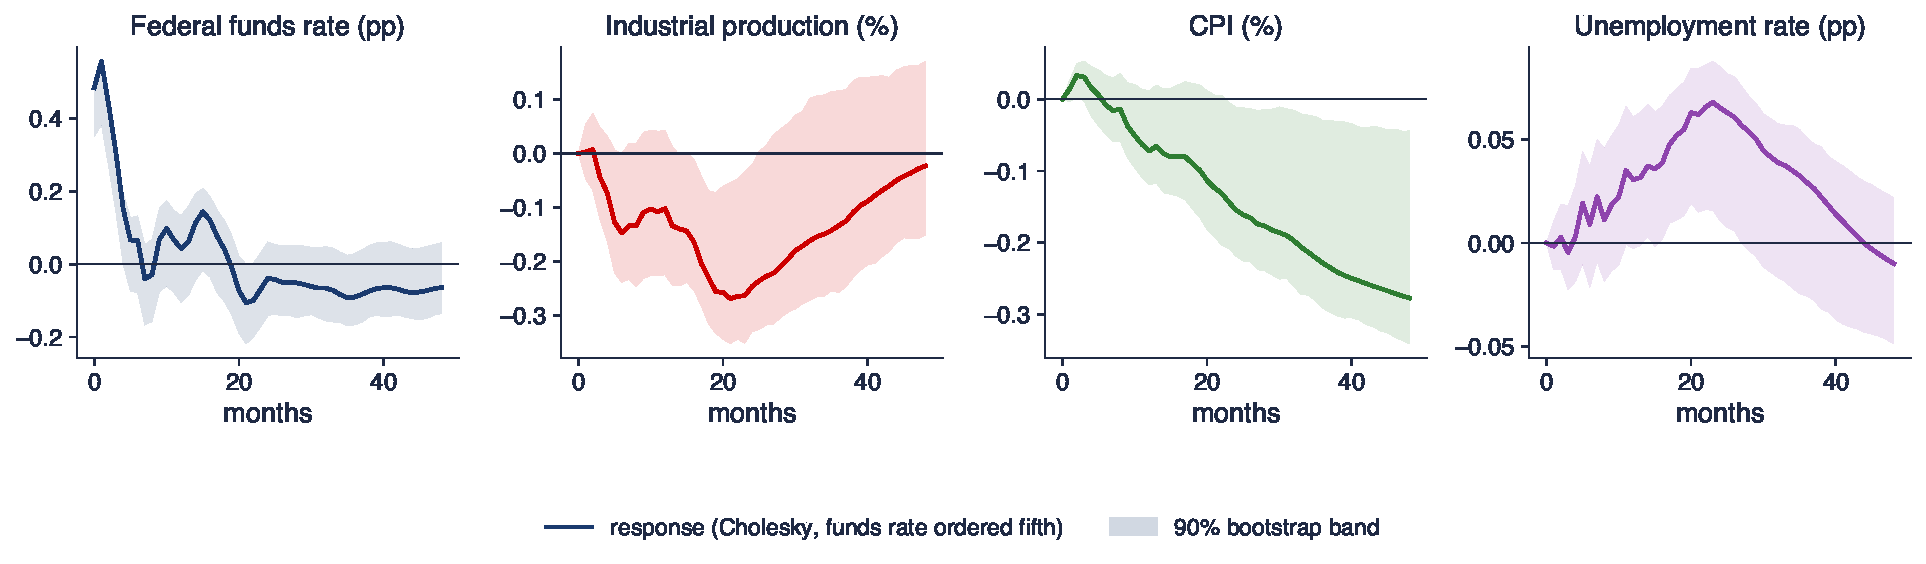
\includegraphics[width=0.97\textwidth,height=0.54\textheight,keepaspectratio]{ats_ch3_cee_irf.pdf}
\end{center}
\vspace{-0.25cm}
\begin{itemize}
    \item Răspunsuri la un șoc al dobînzii federal funds de o abatere standard (0{,}48 pp); benzi bootstrap de 90\%
\end{itemize}
\quantlet{ATS\_ch3\_recursive\_var}{\qlurl{ATS_ch3_recursive_var}}
\end{frame}

\begin{frame}{Interpretarea răspunsurilor CEE}
\itemsize{\small}
\begin{itemize}
    \item Producția industrială scade lent: minimum \ensuremath{-}0{,}27\% după 21 de luni (banda [\ensuremath{-}0{,}35; \ensuremath{-}0{,}05]); șomajul crește cu cel mult 0{,}07 pp
    \begin{itemize}
        \item forma de cocoașă și întîrzierea sînt clasicele „laguri lungi și variabile” (long and variable lags) ale politicii monetare
    \end{itemize}
    \item Prețurile cresc întîi ușor (0{,}033\% după 2 luni), apoi scad la \ensuremath{-}0{,}28\% după patru ani
    \begin{itemize}
        \item creșterea inițială este \textbf{anomalia prețurilor} (price puzzle): Fed înăsprește politica atunci cînd anticipează inflație; prețurile materiilor prime din VAR o reduc, dar nu o elimină
    \end{itemize}
    \item Șocurile monetare explică puțin din producție: 6{,}6\% din varianța erorii de prognoză a IP la 24 de luni
\end{itemize}
\end{frame}

\begin{frame}{Restricții nerecursive pe termen scurt}
\itemsize{\small}
\begin{itemize}
    \item \textbf{Modelul AB} \refLut, \refKL: $Au_t = B\varepsilon_t$; zerouri și valori cunoscute oriunde în $A$ și $B$
    \begin{itemize}
        \item $A$: relațiile contemporane dintre componentele lui $u_t$; $B$: impactul șocurilor; atunci $\Sigma_u = A^{-1}BB'A^{-1\prime}$
        \item estimat prin verosimilitate maximă: maximizăm $-\frac T2\ln|\Sigma_u(A, B)| - \frac T2\mathrm{tr}[\Sigma_u(A, B)^{-1}\hat\Sigma_u]$
        \item $|\cdot|$: determinantul; $\mathrm{tr}$: urma matricei; $\hat\Sigma_u$: matricea de covarianță a reziduurilor formei reduse
        \item restricțiile de supraidentificare se testează cu un test al raportului de verosimilitate față de modelul exact identificat
    \end{itemize}
    \item \textbf{Blanchard--Perotti} \refBP: răspunsul automat al taxelor la producție este o elasticitate \emph{externă} (din legislația fiscală)
    \begin{itemize}
        \item cu această elasticitate fixată, inovația taxelor ajustată ciclic este un instrument pentru coeficienții rămași
        \item cheltuielile publice sînt predeterminate în trimestru (întîrzieri de decizie): o restricție zero cu un argument instituțional
    \end{itemize}
    \item Seminarul 3, A2: o elasticitate cunoscută identifică un sistem $2\times2$ prin variabile instrumentale
\end{itemize}
\end{frame}

\begin{frame}{Limitele ipotezei recursive}
\itemsize{\small}
\begin{itemize}
    \item Simultaneitatea: dobînzile și prețurile activelor reacționează unele la altele în aceeași zi
    \begin{itemize}
        \item nicio ordonare a prețurilor acțiunilor și a dobînzii de politică nu este credibilă la frecvență lunară
    \end{itemize}
    \item Informația omisă: șocul de politică absoarbe prognozele Fed
    \begin{itemize}
        \item șocurile narative \refRR\ curăță modificarea intenționată a dobînzii de prognozele din Greenbook
    \end{itemize}
    \item Dependența de eșantion: după 1983 răspunsurile sînt mai slabe și deseori anormale \refRam
    \begin{itemize}
        \item remediile din secțiunile următoare: restricții mai slabe (semne) sau informație externă (instrumente)
    \end{itemize}
\end{itemize}
\end{frame}

\begin{frame}{Recapitulare: restricții pe termen scurt}
\itemsize{\small}
\begin{itemize}
    \item Cholesky = ipoteze despre momentul reacției; pentru răspunsurile unui șoc contează doar poziția variabilei lui
    \item CEE: producția scade cu o întîrziere de aproximativ 21 de luni; anomalia prețurilor rămîne
    \item Schemele nerecursive folosesc cunoștințe instituționale (elasticități fiscale, întîrzieri de decizie) și pot fi supraidentificate și testate
    \item Zerourile pe termen scurt sînt cel mai puțin credibile exact acolo unde contează mai mult: pe piețele rapide
\end{itemize}
\end{frame}


%=============================================================================
\section{Studiu de caz: șocuri de ofertă și de cerere pe piața petrolului}
%=============================================================================

\begin{frame}{Nu toate șocurile prețului petrolului sînt la fel}
\itemsize{\footnotesize}
\begin{columns}[T]
\begin{column}{0.38\textwidth}
\centering
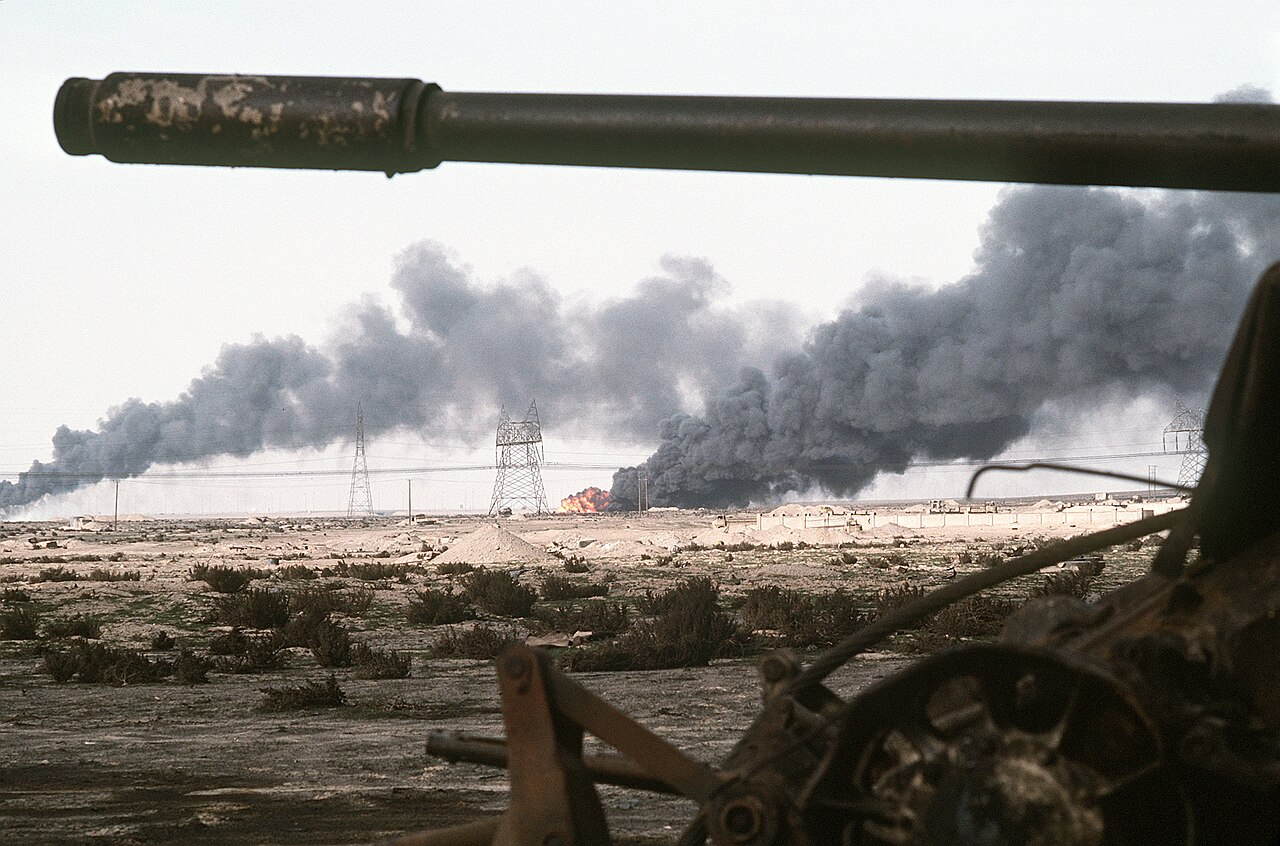
\includegraphics[height=0.36\textheight]{ch3_kuwait_oil_fires_1991.jpg}\\[1mm]
\imgcap{Cîmp petrolier în flăcări, Kuweit, martie 1991}
\imgcredit{https://commons.wikimedia.org/wiki/File:Disabled_Iraqi_T-54A,_T-55,_Type_59_or_Type_69_tank_and_burning_Kuwaiti_oil_field.jpg}{Foto: JO1 Gawlowicz, US Navy (1991); domeniu public; Wikimedia Commons}
\end{column}
\begin{column}{0.60\textwidth}
\begin{itemize}
    \item \refKilB: VAR(24) lunar cu (i) variația procentuală a producției mondiale de țiței, (ii) activitatea reală globală, (iii) logaritmul prețului real al petrolului
    \begin{itemize}
        \item recursiv: oferta de petrol nu răspunde în aceeași lună la cerere (costuri de ajustare); activitatea reală nu răspunde în aceeași lună la cererea specifică petrolului
    \end{itemize}
    \item Trei șocuri: oferta de petrol, cererea agregată, cererea specifică petrolului (de precauție)
    \begin{itemize}
        \item activitatea reală: indicele din \refKilB\ corectat în \refKilC\ (FRED IGREA); prețul: costul de achiziție al țițeiului importat de rafinării, deflatat cu IPC din SUA
    \end{itemize}
    \item Eșantionul nostru începe în 1974 (prima lună a seriei de prețuri), eșantionul efectiv din ianuarie 1976, $T = 384$; extindere pînă în mai 2026
\end{itemize}
\end{column}
\end{columns}
\end{frame}

\begin{frame}{Răspunsuri la șocurile de ofertă și de cerere pe piața petrolului}
\itemsize{\footnotesize}
\begin{center}
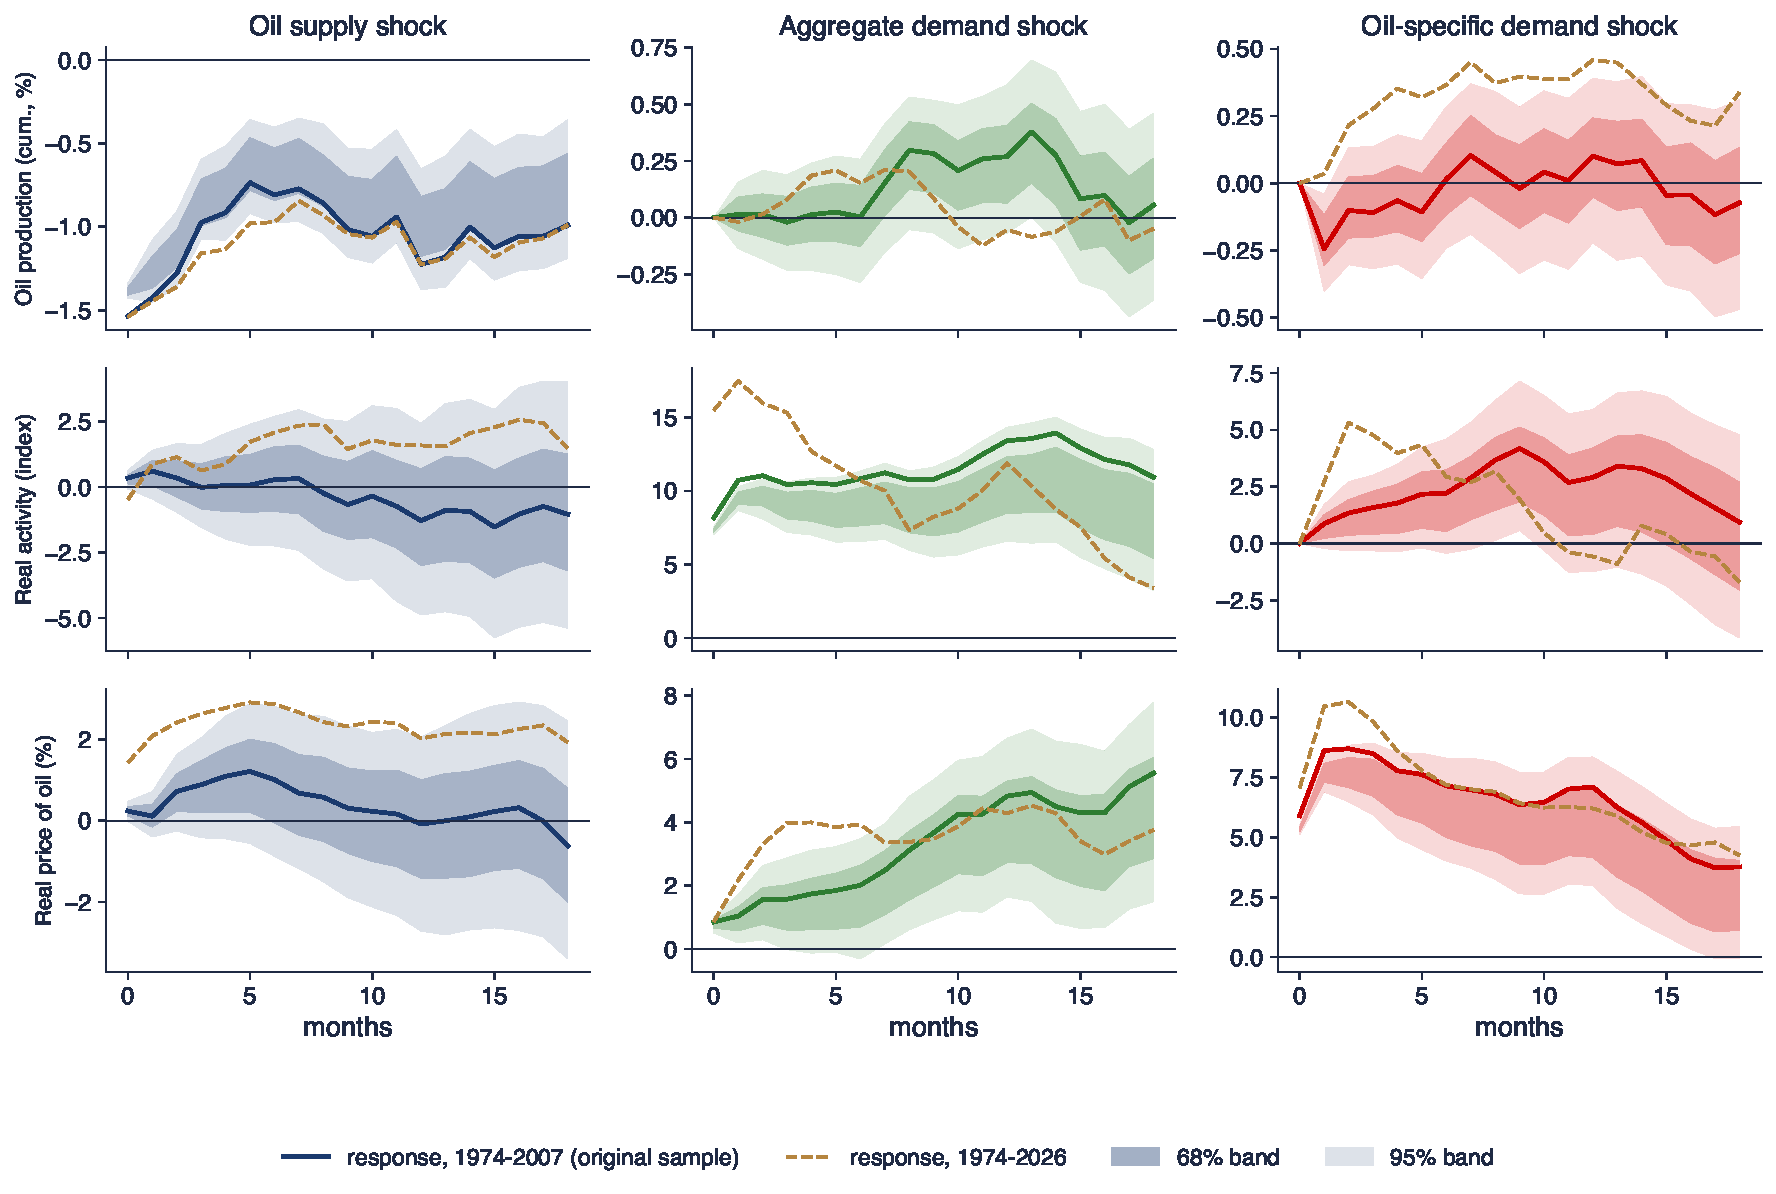
\includegraphics[width=0.97\textwidth,height=0.64\textheight,keepaspectratio]{ats_ch3_kilian_irf.pdf}
\end{center}
\vspace{-0.25cm}
\begin{itemize}
    \item Șocuri de o abatere standard, producția cumulată; benzi bootstrap wild cu design recursiv de 68\% și 95\% \refGoK; linia întreruptă: eșantionul extins pînă în 2026
\end{itemize}
\quantlet{ATS\_ch3\_oil\_shocks}{\qlurl{ATS_ch3_oil_shocks}}
\end{frame}

\begin{frame}{Interpretarea răspunsurilor pe piața petrolului}
\itemsize{\small}
\begin{itemize}
    \item Șocul de ofertă: producția scade cu \ensuremath{-}1{,}5\% la impact, prețul real aproape nu se mișcă (\ensuremath{-}0{,}1\% după 12 luni, banda [\ensuremath{-}2{,}8; 2{,}2])
    \begin{itemize}
        \item în eșantionul extins efectul este mai mare (2{,}0\%): piața de după 2008 reacționează mai mult la veștile despre ofertă
    \end{itemize}
    \item Cererea agregată: o creștere întîrziată și persistentă a prețului (4{,}8\% după 12 luni, banda [1{,}5; 6{,}8])
    \item Cererea specifică petrolului: un salt imediat (5{,}9\%) care persistă (7{,}1\% după 12 luni)
    \item La 60 de luni, șocurile de ofertă explică 1\% din varianța prețului, cererea agregată 64\%, cererea specifică 35\%: prețul petrolului este determinat mai ales de cerere
\end{itemize}
\end{frame}

\begin{frame}{Descompunerea istorică a prețului real al petrolului}
\itemsize{\footnotesize}
\begin{center}
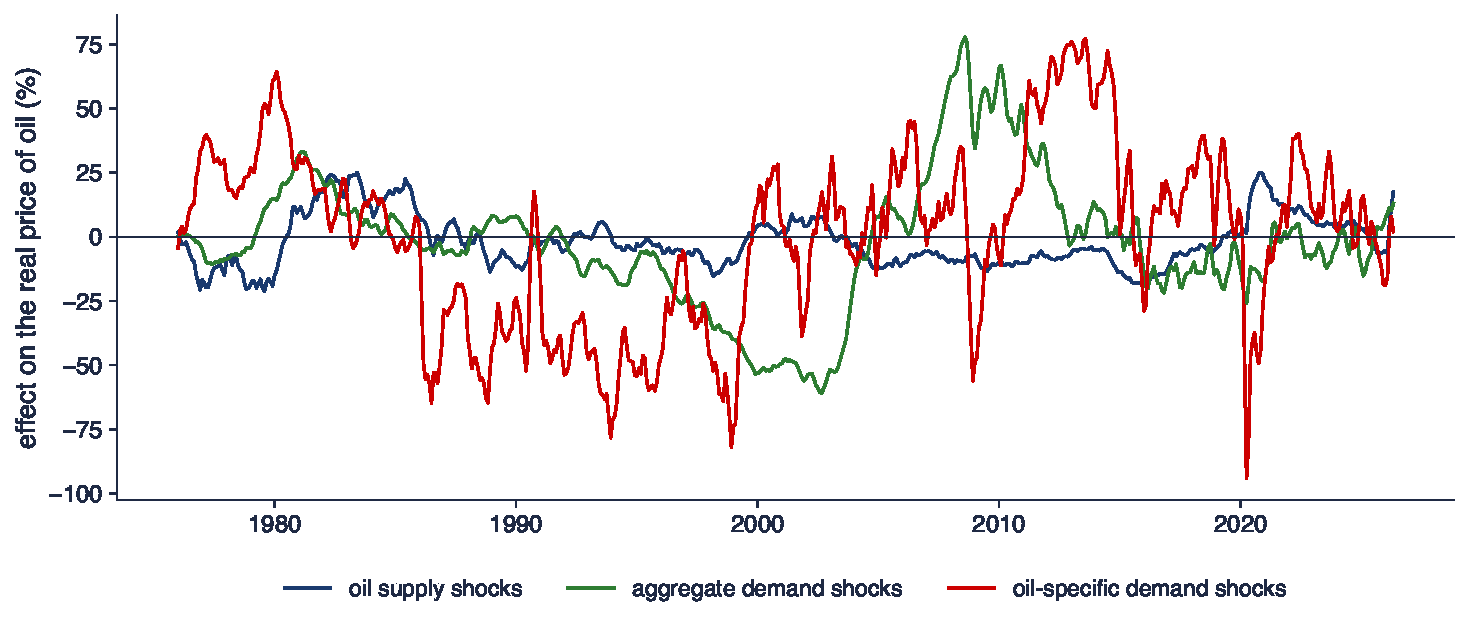
\includegraphics[width=0.97\textwidth,height=0.69\textheight,keepaspectratio]{ats_ch3_kilian_hd.pdf}
\end{center}
\vspace{-0.25cm}
\begin{itemize}
    \item Contribuția cumulată a fiecărui șoc structural, 1976--2026 (VAR(24) recursiv, eșantionul extins); puncte logaritmice $\times 100$
\end{itemize}
\quantlet{ATS\_ch3\_oil\_shocks}{\qlurl{ATS_ch3_oil_shocks}}
\end{frame}

\begin{frame}{Interpretarea descompunerii istorice}
\itemsize{\small}
\begin{itemize}
    \item 2003--mijlocul lui 2008: cererea agregată adaugă 126 de puncte logaritmice, oferta \ensuremath{-}12: boom-ul a fost unul al cererii globale
    \item De la mijlocul lui 2008 la începutul lui 2009: cererea specifică \ensuremath{-}82, cererea agregată \ensuremath{-}35; începutul lui 2020: cererea specifică \ensuremath{-}103
    \item De la mijlocul lui 2021 la mijlocul lui 2022: cererea specifică 43, oferta \ensuremath{-}2: modelul citește saltul din 2022 drept cerere de precauție
    \item Rezervă: restricția zero pentru răspunsul ofertei este puternică; \refBHb\ permit o elasticitate mică, dar nenulă, și găsesc un rol mai mare pentru ofertă
    \begin{itemize}
        \item o descompunere este la fel de bună ca ipoteza de identificare din spatele ei
    \end{itemize}
\end{itemize}
\end{frame}


%=============================================================================
\section{Restricții pe termen lung}
%=============================================================================

\begin{frame}{Blanchard și Quah: multiplicatorul de termen lung (1/2)}
\itemsize{\small}
\begin{itemize}
    \item Pentru $y_t = (\Delta\text{producție}_t, u_t)'$ răspunsurile cumulate sînt
    \begin{itemize}
        \item $\Theta(1) = \sum_h\Theta_h = (I - A_1 - \dots - A_p)^{-1}B_0 = A(1)^{-1}B_0$
        \item aici $u_t$ este rata șomajului; $A(1) = I - A_1 - \dots - A_p$: polinomul VAR evaluat în 1; primul rînd al $\Theta(1)$ este efectul de termen lung asupra \emph{nivelului} producției
    \end{itemize}
    \item Restricția \refBQ: șocurile de cerere nu au efect pe termen lung asupra nivelului producției
    \begin{itemize}
        \item $[\Theta(1)]_{12} = 0$
        \item $[\cdot]_{12}$: elementul din rîndul 1 (producția) și coloana 2 (șocul de cerere)
    \end{itemize}
\end{itemize}
\end{frame}

\begin{frame}{Blanchard și Quah: multiplicatorul de termen lung (2/2)}
\itemsize{\small}
\begin{itemize}
    \item Algoritmul: $\Theta(1)\Theta(1)' = A(1)^{-1}\Sigma_uA(1)^{-1\prime}$ este cunoscut din forma redusă
    \begin{itemize}
        \item luăm factorul Cholesky inferior triunghiular $L$ (zeroul din poziția $(1,2)$), apoi $B_0 = A(1)L$
        \item zeroul este pus pe matricea de termen lung, nu pe matricea de impact; derivarea în \atsapplink{atsapp1}{atssrc1}{Anexă} și în Seminarul 3, A3
    \end{itemize}
    \item Interpretare: „oferta” = toate șocurile cu efecte permanente (tehnologie, oferta de muncă); \refGali\ folosește aceeași idee pentru șocurile tehnologice și orele lucrate
\end{itemize}
\end{frame}

\begin{frame}{Studiu de caz: Blanchard și Quah (1989)}
\itemsize{\small}
\begin{itemize}
    \item Lucrarea: creșterea PNB real în SUA și rata șomajului (bărbați de 20 de ani și peste), trimestrial, VAR(8), 1950:2--1987:4 \refBQ
    \begin{itemize}
        \item tratarea datelor: medii separate ale creșterii producției înainte și după 1973:4 (încetinirea productivității), trend liniar eliminat din șomaj
    \end{itemize}
    \item Replicarea noastră: aceeași specificație pe versiunea actuală a datelor (FRED GNPC96, LNS14000025), $T = 151$; benzi bootstrap de 90\%
    \item Întrebarea: determină șocurile de cerere ciclul economic și cît durează efectele lor?
\end{itemize}
\end{frame}

\begin{frame}{Șocuri de ofertă și de cerere identificate printr-o restricție de termen lung}
\itemsize{\footnotesize}
\begin{center}
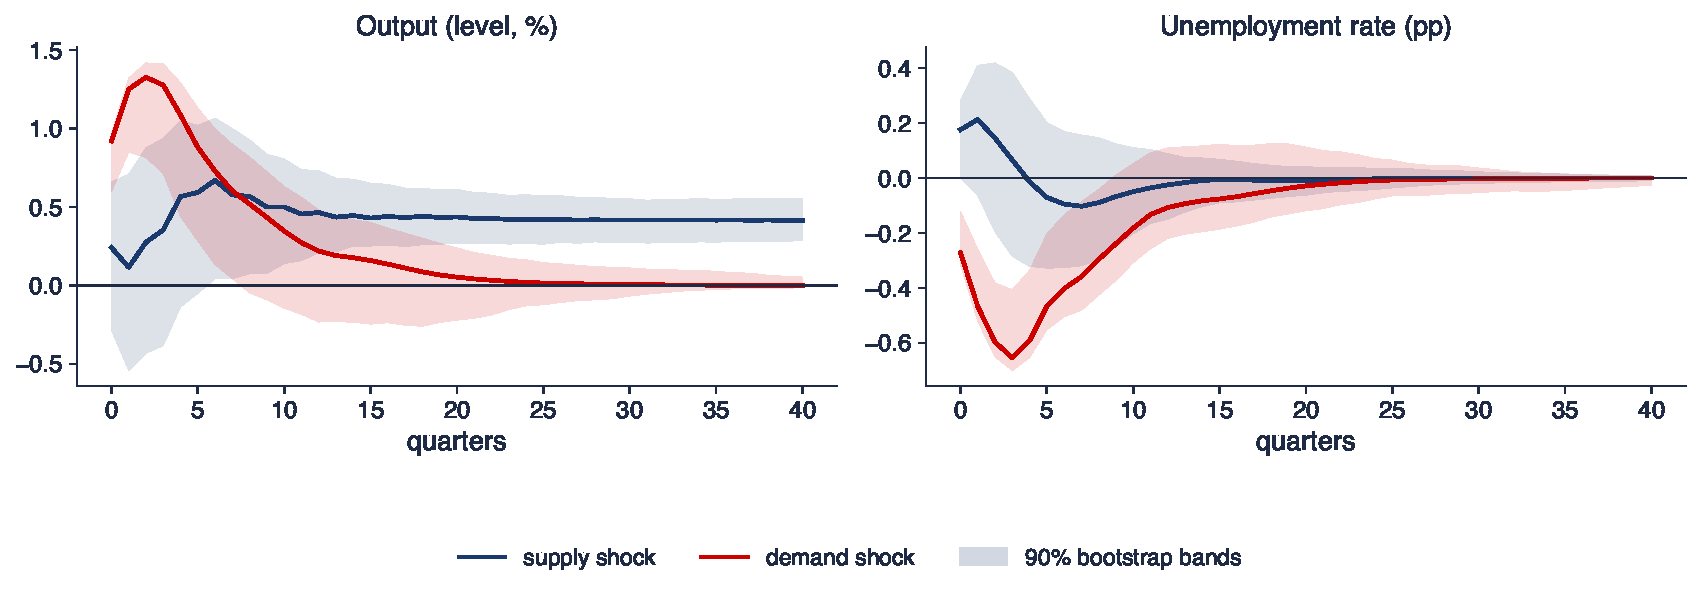
\includegraphics[width=0.97\textwidth,height=0.65\textheight,keepaspectratio]{ats_ch3_bq.pdf}
\end{center}
\vspace{-0.25cm}
\begin{itemize}
    \item Nivelul producției (creșterea cumulată) și șomajul; șocuri de o abatere standard; benzi bootstrap de 90\%
\end{itemize}
\quantlet{ATS\_ch3\_long\_run}{\qlurl{ATS_ch3_long_run}}
\end{frame}

\begin{frame}{Interpretarea răspunsurilor Blanchard--Quah}
\itemsize{\small}
\begin{itemize}
    \item Șocul de cerere: producția atinge un maxim de 1{,}33\% după 2 trimestre și revine la zero prin construcție; șomajul scade cu \ensuremath{-}0{,}65 pp
    \item Șocul de ofertă: producția crește permanent (0{,}42\% după zece ani, banda [0{,}28; 0{,}55]), iar șomajul întîi \emph{crește} (0{,}18 pp)
    \item Șocurile de cerere explică 92\% din varianța nivelului producției la un an și 54\% la zece ani: în acord cu \refBQ, cererea domină la orizonturile ciclului economic
    \item Seminarul 3, B5: fără ruptură și fără trend, ponderile se schimbă radical
\end{itemize}
\end{frame}

\begin{frame}{Fiabilitatea restricțiilor de termen lung}
\itemsize{\small}
\begin{itemize}
    \item \refFL: multiplicatorul de termen lung $A(1)^{-1}$ se estimează imprecis din eșantioane finite
    \begin{itemize}
        \item un șoc cu un efect permanent foarte mic nu se poate distinge de unul tranzitoriu: inferența poate fi distorsionată oricît de mult
        \item comportamentul de rădăcină aproape unitară al șomajului agravează problema
    \end{itemize}
    \item Rezultatele depind de tratarea frecvențelor joase: rupturi în creșterea medie, trenduri, numărul de laguri
    \begin{itemize}
        \item \atschlink{https://danpele.github.io/Advanced-Time-Series/RO/Cursuri/capitol2_rupturi_structurale_modele_neliniare.pdf}{Capitolul 2} testează astfel de rupturi; \atschlink{https://danpele.github.io/Advanced-Time-Series/RO/Cursuri/capitol4_cointegrare_vecm_ardl_panel.pdf}{Capitolul 4} tratează cointegrarea, unde restricțiile de termen lung devin restricții asupra VECM
    \end{itemize}
    \item Folosiți restricțiile de termen lung împreună cu un tabel de sensibilitate, niciodată singure
\end{itemize}
\end{frame}

\begin{frame}{Recapitulare: restricții pe termen lung}
\itemsize{\small}
\begin{itemize}
    \item Restricționăm $\Theta(1) = A(1)^{-1}B_0$ în loc de $B_0$: identificare prin permanență
    \item BQ: cererea domină fluctuațiile producției pe orizontul ciclului, oferta termenul lung
    \item Fragile: tratarea frecvențelor joase și multiplicatorul de termen lung imprecis determină răspunsul
\end{itemize}
\end{frame}


%=============================================================================
\section{Restricții de semn și identificarea pe mulțimi}
%=============================================================================

\begin{frame}{Identificarea prin semne (1/2)}
\itemsize{\small}
\begin{itemize}
    \item Restricționăm doar \textbf{semnele} unor răspunsuri pe anumite orizonturi: un șoc monetar contracționist crește dobînda și scade prețurile \refUhl
    \begin{itemize}
        \item răspunsul de interes (producția) rămîne nerestricționat: o procedură „agnostică”
    \end{itemize}
    \item Algoritmul \refRWZ: extragem o rotație aleatoare $Q$
    \begin{itemize}
        \item extragem $X$ ($n \times n$) cu elemente i.i.d.\ $N(0, 1)$ și calculăm descompunerea QR $X = QR$ ($Q$ ortogonală, $R$ superior triunghiulară)
        \item normalizăm semnele lui $\mathrm{diag}(R)$ să fie pozitive: atunci $Q$ este uniformă (Haar) pe mulțimea matricelor ortogonale
    \end{itemize}
\end{itemize}
\end{frame}

\begin{frame}{Identificarea prin semne (2/2)}
\itemsize{\small}
\begin{itemize}
    \item Acceptăm sau respingem rotația
    \begin{itemize}
        \item calculăm $\Theta_h = \Phi_hPQ$ și păstrăm $Q$ dacă toate semnele sînt respectate; repetăm pentru extrageri ale lui $(A, \Sigma_u)$ din distribuția a posteriori
        \item restricțiile zero împreună cu semne cer algoritmul cu eșantionare de importanță din \refARW
    \end{itemize}
    \item Rezultatul este o \textbf{mulțime} de modele compatibile cu datele și cu restricțiile, nu un punct
\end{itemize}
\end{frame}

\begin{frame}{Restricții de semn în două dimensiuni}
\itemsize{\footnotesize}
\begin{center}
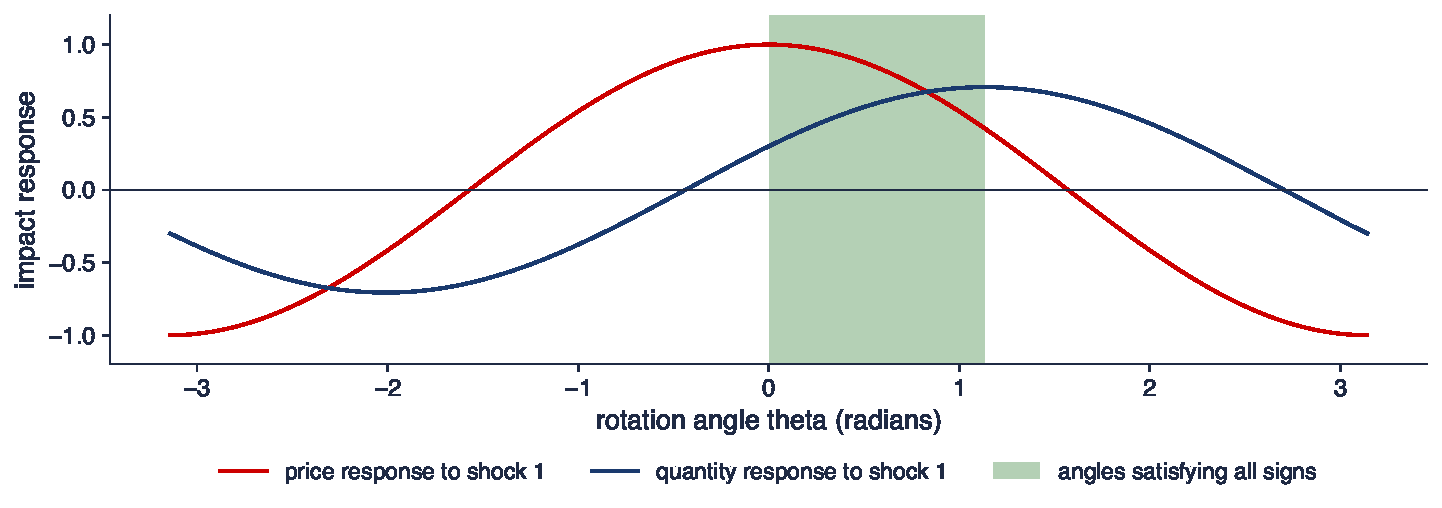
\includegraphics[width=0.97\textwidth,height=0.65\textheight,keepaspectratio]{ats_ch3_rotation.pdf}
\end{center}
\vspace{-0.25cm}
\begin{itemize}
    \item Inovații ale prețului și cantității cu varianțele 1 și 0,5 și covarianța 0,3; răspunsurile la impact $P(\cos\theta, \sin\theta)'$ la șocul 1 cînd variază unghiul de rotație; cererea: $(+, +)$, oferta: $(+, -)$
\end{itemize}
\quantlet{ATS\_ch3\_sign\_restrictions}{\qlurl{ATS_ch3_sign_restrictions}}
\end{frame}

\begin{frame}{Interpretarea mulțimii de rotații}
\itemsize{\small}
\begin{itemize}
    \item Toate semnele sînt respectate pentru $\theta \in (0; 1{,}13)$, 18\% din cerc: un interval întreg de modele este la fel de compatibil cu datele
    \item Efectul la impact al cererii asupra cantității se află oriunde în $[0{,}30; 0{,}71]$: \textbf{mulțimea identificată}
    \item O extragere uniformă a lui $\theta$ pune o distribuție a priori pe acest interval: distribuția a posteriori în interiorul mulțimii este cea a priori, nu informație din date
    \begin{itemize}
        \item acesta este argumentul din \refBHa: extragerile Haar sînt informative pentru răspunsuri
    \end{itemize}
\end{itemize}
\end{frame}

\begin{frame}{Studiu de caz: Uhlig (2005)}
\itemsize{\small}
\begin{itemize}
    \item Lucrarea: VAR(12) lunar pentru SUA cu șase variabile, fără termen liber, 1965:1--2003:12; un șoc contracționist crește dobînda federal funds și scade prețurile, prețurile materiilor prime și rezervele neîmprumutate în lunile 0--5 \refUhl
    \begin{itemize}
        \item producția nu este restricționată: întrebarea este chiar semnul ei
    \end{itemize}
    \item Replicarea noastră: aceleași restricții și același eșantion; IP și IPC înlocuiesc PIB-ul și deflatorul interpolate lunar din lucrare (datele din \refRam)
    \begin{itemize}
        \item distribuție a posteriori Normal--inverse-Wishart cu prior plat, 1\,000 de extrageri, vectori de impuls Haar; acceptate: 985 de extrageri; la estimația OLS, 4{,}1\% dintre rotații respectă semnele
    \end{itemize}
    \item Întrebarea: scade un șoc monetar contracționist producția atunci cînd producția este lăsată liberă?
\end{itemize}
\end{frame}

\begin{frame}{Un șoc de politică monetară agnostic}
\itemsize{\footnotesize}
\begin{center}
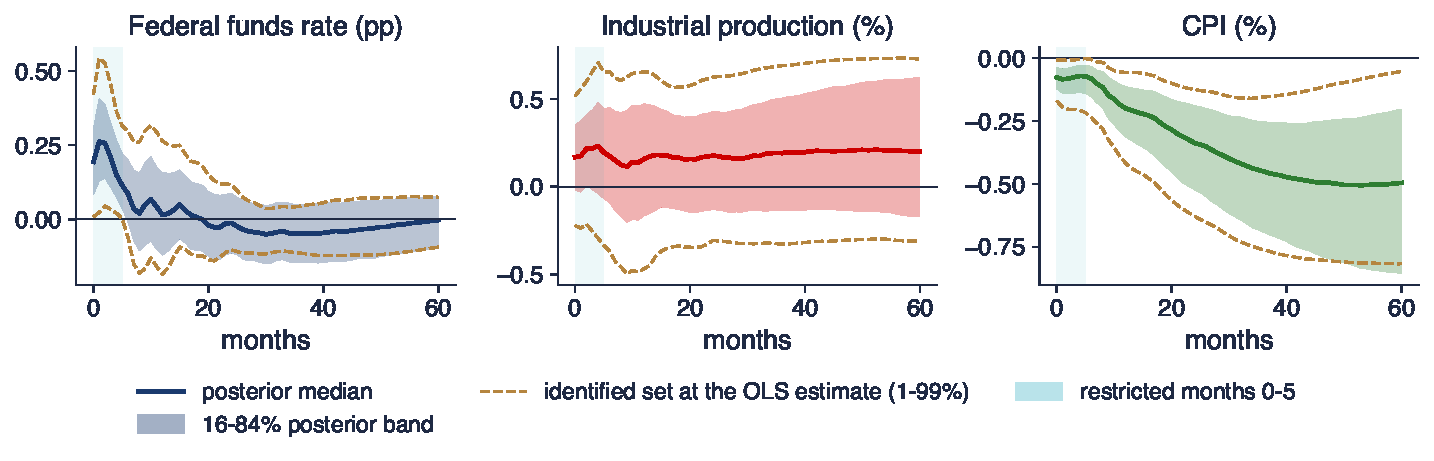
\includegraphics[width=0.97\textwidth,height=0.59\textheight,keepaspectratio]{ats_ch3_uhlig.pdf}
\end{center}
\vspace{-0.25cm}
\begin{itemize}
    \item Șoc de o abatere standard; mediana a posteriori și banda 16--84\%; linia întreruptă: intervalul 1--99\% al mulțimii identificate la estimația OLS; zona colorată: lunile restricționate
\end{itemize}
\quantlet{ATS\_ch3\_sign\_restrictions}{\qlurl{ATS_ch3_sign_restrictions}}
\end{frame}

\begin{frame}{Interpretarea răspunsurilor agnostice}
\itemsize{\small}
\begin{itemize}
    \item Producția după 12 luni: mediana 0{,}16\%, banda [\ensuremath{-}0{,}17; 0{,}47]; 32\% dintre extrageri negative: nicio dovadă că producția scade
    \item Mulțimea identificată la estimația OLS acoperă [\ensuremath{-}0{,}47; 0{,}66]: datele împreună cu semnele nu pot determina semnul producției
    \item Prețurile scad persistent (\ensuremath{-}0{,}34\% după 24 de luni), fără anomalia prețurilor, pentru că restricția o exclude
    \item Concluzia lui Uhlig, confirmată: neutralitatea șocurilor de politică monetară pentru producție nu este incompatibilă cu datele
\end{itemize}
\end{frame}

\begin{frame}{Inferența sub identificarea pe mulțimi}
\itemsize{\small}
\begin{itemize}
    \item Mediana a posteriori nu este un model structural: la fiecare orizont poate proveni dintr-o altă rotație \refFP
    \begin{itemize}
        \item raportați un singur model admisibil apropiat de mediană (median target) sau, mai bine, întreaga mulțime
    \end{itemize}
    \item Distribuția a priori Haar este informativă pentru răspunsuri \refBHa; \refGKi\ propun Bayes robust: raportați intervalul mediilor a posteriori peste toate distribuțiile a priori pentru $Q$
    \begin{itemize}
        \item banda robustă este mai largă și mai prudentă: separă ce spun datele de ce spune distribuția a priori
    \end{itemize}
    \item Restrîngeți mulțimea cu mai multă informație: mai multe semne, zerouri \refARW, evenimente narative, limite pentru elasticități \refBHb
\end{itemize}
\end{frame}

\begin{frame}{Restricții narative}
\itemsize{\footnotesize}
\begin{columns}[T]
\begin{column}{0.36\textwidth}
\centering

\includegraphics[height=0.34\textheight]{ch3_volcker_2014.jpg}\\[1mm]
\imgcap{Paul Volcker, președintele Fed 1979--1987}
\imgcredit{https://commons.wikimedia.org/wiki/File:Paul_Volcker_-_2014_(13896577879)_(cropped).jpg}{Foto: Federal Reserve (2014); domeniu public; Wikimedia Commons}
\end{column}
\begin{column}{0.62\textwidth}
\begin{itemize}
    \item \refADRR: restricționăm șocurile structurale la anumite date, nu răspunsurile
    \begin{itemize}
        \item octombrie 1979 (trecerea lui Volcker la țintirea rezervelor) a fost un șoc pozitiv de politică monetară
        \item și a fost principalul factor al modificării neașteptate a dobînzii federal funds în acea lună
    \end{itemize}
    \item Cîteva evenimente credibile elimină majoritatea rotațiilor lăsate de restricțiile de semn singure
    \begin{itemize}
        \item verosimilitatea trebuie reponderată cu probabilitatea respectării restricției narative (eșantionare de importanță)
    \end{itemize}
    \item Cu restricții narative, producția scade după un șoc contracționist, spre deosebire de mulțimea agnostică
\end{itemize}
\end{column}
\end{columns}
\end{frame}

\begin{frame}{Identificarea prin heteroscedasticitate}
\itemsize{\small}
\begin{itemize}
    \item Dacă varianțele șocurilor structurale se schimbă între regimuri, iar $B_0$ rămîne fix: $\Sigma_1 = B_0B_0'$, $\Sigma_2 = B_0\Lambda B_0'$, $\Lambda$ diagonală \refRig
    \begin{itemize}
        \item $\Sigma_1, \Sigma_2$: matricele de covarianță ale formei reduse în cele două regimuri; $\Lambda = \mathrm{diag}(\lambda_1, \dots, \lambda_n)$: varianțele relative ale șocurilor în regimul 2
        \item atunci $\Sigma_1^{-1}\Sigma_2 = B_0^{-1\prime}\Lambda B_0'$: coloanele lui $B_0$ rezultă dintr-o descompunere în valori proprii, unică dacă $\lambda_i$ sînt distincte
        \item regimuri: date cunoscute (crize, anunțuri de politică) sau estimate (Markov switching, GARCH) \refLL
    \end{itemize}
    \item Identificarea statistică dă șocuri fără nume: etichetarea lor cere tot argumente economice (semne)
    \begin{itemize}
        \item ipoteza că $B_0$ este același în ambele regimuri este puternică și se poate testa doar parțial
    \end{itemize}
    \item Seminarul 3, A8 recuperează $B_0$ din două matrice de covarianță de mînă; \atschlink{https://danpele.github.io/Advanced-Time-Series/RO/Cursuri/capitol7_modele_schimbare_regim.pdf}{Capitolul 7} dezvoltă modelele cu schimbare de regim
\end{itemize}
\end{frame}

\begin{frame}{Recapitulare: restricții de semn și identificarea pe mulțimi}
\itemsize{\small}
\begin{itemize}
    \item Semnele dau o mulțime de modele; raportați mulțimea, nu doar mediana a posteriori
    \item Uhlig: cu prețurile, dobînzile și rezervele restricționate, producția poate evolua în orice sens
    \item Distribuția a priori Haar contează; Bayes robust și restricțiile narative fac concluziile mai precise, fără a le exagera
    \item Heteroscedasticitatea identifică statistic; economia dă încă numele șocurilor
\end{itemize}
\end{frame}


%=============================================================================
\section{Instrumente externe}
%=============================================================================

\begin{frame}{Modelul proxy SVAR (1/2)}
\itemsize{\small}
\begin{itemize}
    \item O variabilă externă $z_t$ (proxy), corelată cu șocul de interes $\varepsilon_{1t}$ și cu niciun alt șoc
    \begin{itemize}
        \item \textbf{relevanța}: $\E z_t\varepsilon_{1t} = \alpha \ne 0$; \textbf{exogenitatea}: $\E z_t\varepsilon_{jt} = 0$ pentru $j \ne 1$
    \end{itemize}
    \item Atunci covarianța reziduurilor cu proxy-ul este proporțională cu coloana de impact $b_1$
    \begin{itemize}
        \item $\E u_tz_t = B_0\E\varepsilon_tz_t = \alpha b_1$ (derivarea în \atsapplink{atsapp2}{atssrc2}{Anexă})
        \item $b_1$: prima coloană a lui $B_0$, efectele la impact ale șocului 1 asupra tuturor celor $n$ variabile
    \end{itemize}
\end{itemize}
\end{frame}

\begin{frame}{Modelul proxy SVAR (2/2)}
\itemsize{\small}
\begin{itemize}
    \item Normalizăm $b_{11} = 1$ (sau o creștere a dobînzii de 25 bp) și estimăm impacturile relative \refSWb, \refMR
    \begin{itemize}
        \item $b_{i1}/b_{11} = \E(u_{it}z_t)/\E(u_{1t}z_t)$
        \item $b_{i1}$: impactul asupra variabilei $i$; numeric, o regresie 2SLS a lui $u_{it}$ pe $u_{1t}$ cu instrumentul $z_t$
    \end{itemize}
    \item Răspunsurile $\Theta_{h,\cdot1} = \Phi_hb_1$: prima coloană a lui $\Theta_h$
    \begin{itemize}
        \item proxy-ul poate fi zgomotos, scurt sau disponibil doar pe un subeșantion
    \end{itemize}
    \item Se identifică o singură coloană a lui $B_0$, fără nicio restricție zero
\end{itemize}
\end{frame}

\begin{frame}{Identificarea politicii monetare la frecvență înaltă}
\itemsize{\small}
\begin{itemize}
    \item Surpriza = modificarea dobînzilor implicite din futures într-o fereastră îngustă (30 de minute) în jurul unui anunț FOMC \refKut, \refGSS
    \begin{itemize}
        \item în 30 de minute nu se întîmplă nimic altceva sistematic: exogenitate prin construcție
        \item FF4: contractul futures federal funds peste trei luni; surprinde atît deciziile curente, cît și forward guidance \refGK
    \end{itemize}
    \item Complicații: \textbf{efectul informațional} \refNS: o înăsprire poate semnala vești bune despre economie
    \begin{itemize}
        \item \refJK\ separă șocurile pure de politică de cele informaționale prin co-mișcarea dobînzilor și a prețurilor acțiunilor (restricții de semn asupra surprizelor)
        \item surprizele sînt previzibile din știrile macro anterioare \refBS: ortogonalizați-le înainte de folosire
    \end{itemize}
\end{itemize}
\end{frame}

\begin{frame}{Studiu de caz: Gertler și Karadi (2015)}
\itemsize{\small}
\begin{itemize}
    \item Lucrarea: randamentul titlurilor de stat la 1 an ca indicator de politică (surprinde forward guidance), log IP, log IPC și prima de risc excedentară a obligațiunilor (\refGZ); VAR(12), 1979:7--2012:6 \refGK
    \begin{itemize}
        \item instrumentul: surprizele FF4, lunar, 1991:1--2012:6; reziduurile eșantionului complet sînt folosite în regresia pe proxy pe perioada comună
    \end{itemize}
    \item Replicarea noastră: aceleași variabile, același eșantion și același instrument (fișierele de replicare din \refRam), $T = 384$, $258$ de luni cu instrument
    \begin{itemize}
        \item prima etapă: $F$ robust $= 17{,}7$ (homoscedastic 21{,}9), $R^2 = 7{,}8\%$; benzi bootstrap pe blocuri mobile de 90\% \refJL
    \end{itemize}
    \item Întrebarea: mișcă o surpriză de politică prima de risc a creditului și ce efect are asupra activității?
\end{itemize}
\end{frame}

\begin{frame}{Un șoc de politică monetară identificat cu surprizele FF4}
\itemsize{\footnotesize}
\begin{center}
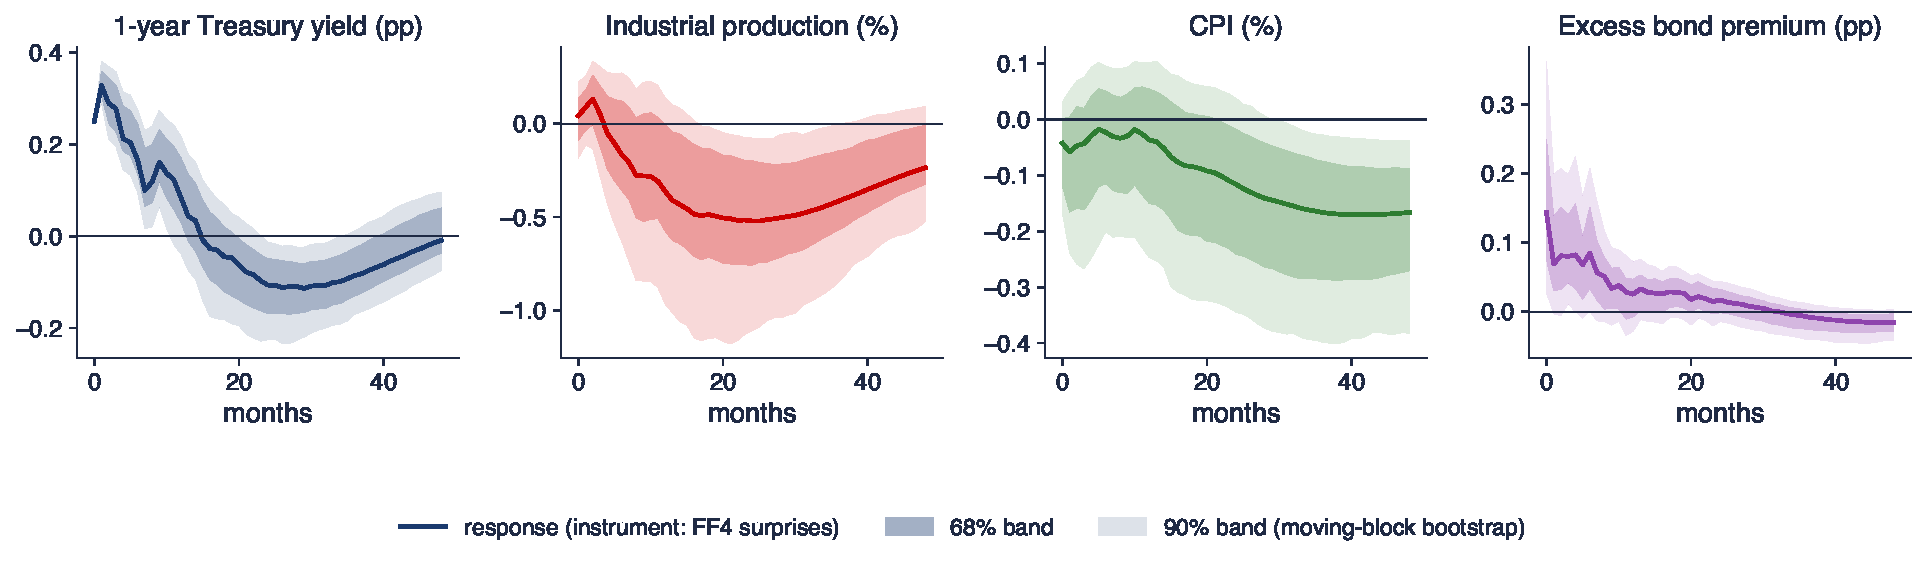
\includegraphics[width=0.97\textwidth,height=0.54\textheight,keepaspectratio]{ats_ch3_gk.pdf}
\end{center}
\vspace{-0.25cm}
\begin{itemize}
    \item Șoc normalizat să crească randamentul la 1 an cu 25 bp la impact; benzi bootstrap pe blocuri mobile de 68\% și 90\%
\end{itemize}
\quantlet{ATS\_ch3\_proxy\_svar}{\qlurl{ATS_ch3_proxy_svar}}
\end{frame}

\begin{frame}{Interpretarea modelului proxy SVAR}
\itemsize{\small}
\begin{itemize}
    \item Prima de risc excedentară crește cu 0{,}14 pp la impact (banda [0{,}03; 0{,}35]): politica monetară acționează prin costul creditului, în acord cu \refGK
    \item IP ajunge la \ensuremath{-}0{,}52\% după 25 de luni (banda [\ensuremath{-}1{,}05; \ensuremath{-}0{,}12]); IPC este \ensuremath{-}0{,}12\% după doi ani (banda [\ensuremath{-}0{,}34; 0{,}04]), fără anomalia prețurilor
    \item $F = 17{,}7$ trece pragul empiric $F > 10$, dar răspunsul prețurilor este imprecis: benzile robuste la instrumente slabe sînt mai largi \refMSW
\end{itemize}
\end{frame}

\begin{frame}{Inferența cu un instrument extern}
\itemsize{\small}
\begin{itemize}
    \item Instrumente slabe: cînd $\alpha$ este mic, raportul $\E(u_iz)/\E(u_1z)$ se estimează prost, iar benzile prin metoda delta au acoperire prea mică
    \begin{itemize}
        \item statistica $F$ din prima etapă: statistica $F$ a regresiei lui $u_{1t}$ pe $z_t$; măsoară tăria instrumentului
    \end{itemize}
    \item Remedii
    \begin{itemize}
        \item \refMSW: mulțimi de încredere de tip Anderson--Rubin, valabile pentru orice tărie a instrumentului; pot fi nemărginite
        \item raportați statistica $F$ din prima etapă cu varianță HAC; regula $F > 10$ este o euristică, nu un test
    \end{itemize}
    \item Bootstrap: bootstrap-ul wild din \refMR\ nu este valid pentru proxy SVAR; folosiți bootstrap-ul pe blocuri mobile al reziduurilor și al instrumentului împreună \refJL
    \begin{itemize}
        \item blocul păstrează dependența dintre pătratul șocului și instrument
    \end{itemize}
    \item Seminarul 3, A5 calculează de mînă impacturile relative și $F$; C1 construiește o mulțime Anderson--Rubin pentru România
\end{itemize}
\end{frame}

\begin{frame}{Recapitulare: instrumente externe}
\itemsize{\small}
\begin{itemize}
    \item Relevanța și exogenitatea unui proxy identifică o coloană a lui $B_0$, fără zerouri
    \item Surprizele de frecvență înaltă sînt cele mai bune proxy-uri disponibile; verificați efectul informațional și previzibilitatea
    \item GK replicat: prima de risc a creditului crește, producția scade; $F = 17{,}7$
    \item Folosiți mulțimi robuste la instrumente slabe și bootstrap-ul pe blocuri
\end{itemize}
\end{frame}


%=============================================================================
\section{Inferența pentru funcțiile de răspuns la impuls}
%=============================================================================

\begin{frame}{Metoda delta și limitele ei}
\itemsize{\small}
\begin{itemize}
    \item $\hat\Theta_h = g(\hat\beta, \hat\sigma)$ este o funcție netedă de estimațiile VAR: $\sqrt T(\hat\Theta_h - \Theta_h) \to N(0, G\Sigma G')$ \refLut
    \begin{itemize}
        \item $\hat\beta$: coeficienții VAR; $\hat\sigma$: elementele distincte ale lui $\hat\Sigma_u$; $\Sigma$: covarianța lor asimptotică comună
        \item $G = \partial g/\partial(\beta, \sigma)$: jacobianul, în formă închisă; rapid, dar benzile sînt simetrice
    \end{itemize}
    \item Eșuează exact unde avem cea mai mare nevoie de ea
    \begin{itemize}
        \item în apropierea rădăcinilor unitare și la orizonturi lungi distribuția lui $\hat\Theta_h$ este asimetrică și ne-Normală
        \item covarianța $G\Sigma G'$ poate fi singulară (de exemplu cînd un răspuns este zero prin construcție)
        \item estimațiile OLS ale pantelor sînt deplasate spre zero în eșantioane mici, deci răspunsurile scad prea repede
    \end{itemize}
    \item De aici bootstrap-ul și corecția deplasării
\end{itemize}
\end{frame}

\begin{frame}{Scheme bootstrap pentru VAR}
\itemsize{\small}
\begin{itemize}
    \item \textbf{Pe reziduuri (design recursiv)}: reeșantionăm $\hat u_t$ i.i.d., reconstruim $y^*_t$ recursiv din VAR-ul estimat, reestimăm, identificăm, repetăm
    \begin{itemize}
        \item valid cu inovații i.i.d.; intervalul percentilelor (sau Hall) al celor $B$ răspunsuri dă banda
    \end{itemize}
    \item \textbf{Wild}: $u^*_t = \eta_t\hat u_t$, $\eta_t = \pm1$ cu probabilitatea $1/2$: robust la heteroscedasticitate condiționată \refGoK
    \begin{itemize}
        \item folosit pentru VAR-ul petrolului: piețele de materii prime au volatility clustering
    \end{itemize}
    \item \textbf{Pe blocuri mobile}: reeșantionăm blocuri de valori consecutive $(\hat u_t, z_t)$; necesar ori de cîte ori contează momentele de ordin superior (proxy SVAR) \refJL
    \begin{itemize}
        \item lungimea blocului de ordinul $T^{1/4}$; \atschlink{https://danpele.github.io/Advanced-Time-Series/RO/Cursuri/capitol0_recapitulare_inferenta.pdf}{Capitolul 0} a tratat alegerea ei
    \end{itemize}
\end{itemize}
\end{frame}

\begin{frame}{Bootstrap-ul cu corecția deplasării al lui Kilian}
\itemsize{\small}
\begin{itemize}
    \item \refKilA: (1) estimăm prin bootstrap deplasarea $\hat b = \bar A^* - \hat A$; (2) corectăm $\tilde A = \hat A - \hat b$, micșorînd corecția dacă $\tilde A$ nu este staționar; (3) aplicăm din nou bootstrap-ul pornind de la $\tilde A$ și corectăm fiecare replicare
    \begin{itemize}
        \item $\hat A$: estimația MCMMP a coeficienților VAR; $\bar A^*$: media estimațiilor bootstrap; $\tilde A$: estimația corectată pentru deplasare
        \item „bootstrap după bootstrap” recentrează distribuția acolo unde deplasarea OLS este mare: serii persistente, eșantioane scurte
    \end{itemize}
    \item VAR-ul petrolului: deplasarea absolută medie 0{,}009 pe coeficient; cea mai mare rădăcină 0{,}994 înainte și 0{,}9999 după corecția (micșorată)
    \begin{itemize}
        \item răspunsul prețului după 12 luni la cererea specifică: 7{,}11\% (OLS), 7{,}34\% (corectat), banda [3{,}4; 9{,}1]; la cererea agregată: 4{,}83\% și 4{,}95\%
    \end{itemize}
    \item Corecția face răspunsurile mai persistente; cînd VAR-ul în niveluri are o rădăcină peste unu, regula lui Kilian îl lasă necorectat (VAR-ul pentru România, secțiunea 9)
\end{itemize}
\end{frame}

\begin{frame}{Benzi punctuale și benzi simultane}
\itemsize{\small}
\begin{itemize}
    \item O bandă punctuală de 90\% acoperă $\Theta_h$ la fiecare $h$ separat; întreaga traiectorie se află în ea cu o probabilitate mult mai mică
    \begin{itemize}
        \item întrebările despre \emph{formă} („producția scade doi ani”) cer benzi simultane \refMOPa
        \item banda sup-$t$: înmulțim erorile standard punctuale cu cuantila $1 - \alpha$ a lui $\max_h|t_h|$ din bootstrap
        \item $t_h$: răspunsul bootstrap la orizontul $h$ minus estimația, împărțit la eroarea lui standard; $\max_h|t_h|$: cea mai mare abatere pe întreaga traiectorie
    \end{itemize}
    \item Benzile bayesiene (cuantile a posteriori) răspund la o altă întrebare: afirmații probabilistice date fiind distribuțiile a priori
    \begin{itemize}
        \item \atschlink{https://danpele.github.io/Advanced-Time-Series/RO/Cursuri/capitol5_bvar_modele_factoriale_nowcasting.pdf}{Capitolul 5} le construiește cu distribuții a priori Minnesota și Normal--inverse-Wishart; la identificarea pe mulțimi ele amestecă distribuția a priori și datele (secțiunea anterioară)
    \end{itemize}
    \item Precizați întotdeauna: punctuală sau simultană, frecventistă sau bayesiană, nivelul (68\%, 90\%, 95\%)
\end{itemize}
\end{frame}

\begin{frame}{Recapitulare: inferența pentru răspunsurile la impuls}
\itemsize{\small}
\begin{itemize}
    \item Benzile prin metoda delta sînt simetrice și eșuează în apropierea rădăcinilor unitare
    \item Bootstrap-ul pe reziduuri, wild și pe blocuri corespunde cazurilor i.i.d., heteroscedastic și proxy
    \item Corecția lui Kilian elimină deplasarea din eșantioane mici; nu se aplică estimațiilor explozive
    \item Întrebările despre formă cer benzi simultane; benzile bayesiene vin în \atschlink{https://danpele.github.io/Advanced-Time-Series/RO/Cursuri/capitol5_bvar_modele_factoriale_nowcasting.pdf}{Capitolul 5}
\end{itemize}
\end{frame}


%=============================================================================
\section{Proiecții locale}
%=============================================================================

\begin{frame}{Proiecțiile locale}
\itemsize{\small}
\begin{itemize}
    \item \refJorda: o regresie pentru fiecare orizont, $y_{i,t+h} = \mu_h + \beta_hx_t + \gamma_h'w_t + \xi_{t+h}$, $h = 0, 1, \dots, H$
    \begin{itemize}
        \item $y_{i,t+h}$: variabila $i$, la $h$ perioade după șoc; $\mu_h$: un termen liber; $\xi_{t+h}$: eroarea de proiecție; $H$: orizontul maxim
        \item $x_t$: șocul (sau variabila de politică cu controalele $w_t$ care o fac practic aleatoare); $\hat\beta_h$ este răspunsul la impuls
        \item nicio iterare a unui model: o dinamică greșit specificată nu se acumulează de la un orizont la altul
    \end{itemize}
    \item Eroarea $\xi_{t+h}$ este autocorelată (cel puțin MA($h - 1$)): erori standard HAC cu $h + 1$ laguri, sau
    \begin{itemize}
        \item \textbf{lag augmentation} (laguri suplimentare) \refMOPb: adăugăm încă un lag al controalelor și folosim erori Eicker--Huber--White; valid uniform după persistență, chiar lîngă o rădăcină unitară
    \end{itemize}
    \item Flexibile: termenii neliniari, dependența de stare, datele panel și variabilele cumulate intră toate ca regresori
\end{itemize}
\end{frame}

\begin{frame}{LP și VAR estimează aceleași răspunsuri}
\itemsize{\small}
\begin{itemize}
    \item \refPW: în populație, o LP cu $p$ laguri ale tuturor variabilelor drept controale și un VAR($p$) cu aceeași ordonare dau răspunsuri \emph{identice} pînă la orizontul $p$ (\atsapplink{atsapp3}{atssrc3}{Anexă})
    \begin{itemize}
        \item cu laguri nerestricționate ($p \to \infty$) coincid la toate orizonturile: alegerea privește estimarea, nu identificarea
        \item orice schemă de identificare VAR (recursivă, instrument extern) are un echivalent LP și invers
    \end{itemize}
    \item În eșantioane finite diferă: VAR-ul extrapolează primele $p$ autocovarianțe, LP folosește direct covarianța la $h$ pași
    \begin{itemize}
        \item slide-ul următor cuantifică această diferență
    \end{itemize}
\end{itemize}
\end{frame}

\begin{frame}{Deplasare și varianță: LP comparat cu VAR (simulare)}
\itemsize{\footnotesize}
\begin{center}
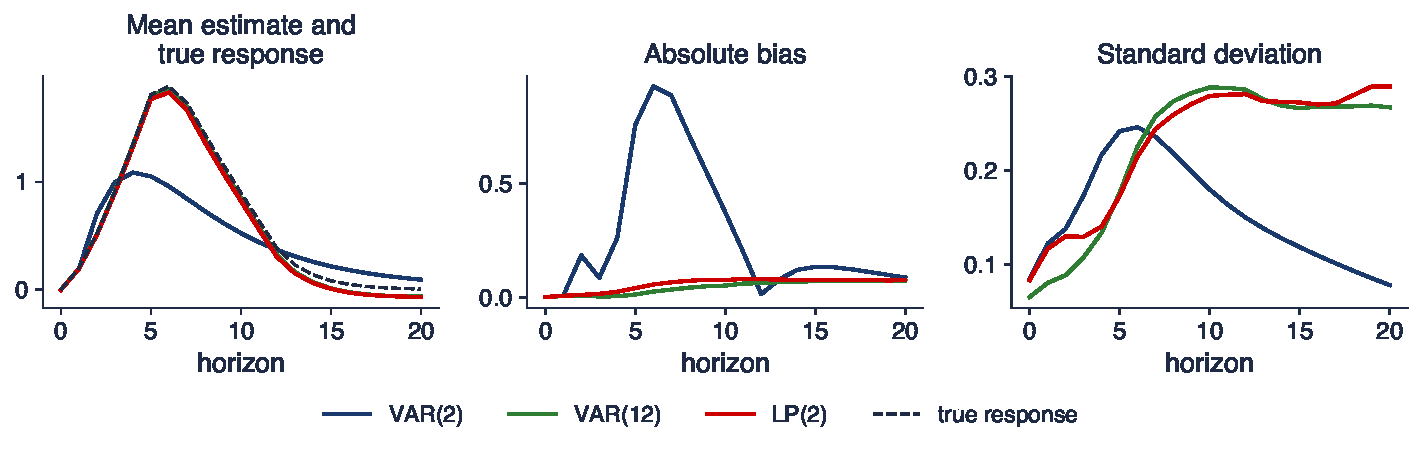
\includegraphics[width=0.97\textwidth,height=0.58\textheight,keepaspectratio]{ats_ch3_lp_sim.pdf}
\end{center}
\vspace{-0.25cm}
\begin{itemize}
    \item DGP: $x_t = 0{,}5x_{t-1} + e_t$, $y_t = 0{,}6y_{t-1} + \sum_{j=0}^{11}\psi_je_{t-j} + u_t$ ($\psi_j$ în formă de cocoașă), $T = 240$, 500 de replicări; $e_t, u_t$: zgomote albe independente; un VAR(2) este greșit specificat
\end{itemize}
\quantlet{ATS\_ch3\_lp\_vs\_var}{\qlurl{ATS_ch3_lp_vs_var}}
\end{frame}

\begin{frame}{Interpretarea compromisului deplasare--varianță}
\itemsize{\small}
\begin{itemize}
    \item La $h = 8$ (răspunsul adevărat 1{,}44): deplasarea VAR(2) 0{,}71, a LP(2) 0{,}07; RMSE 0{,}74 și 0{,}27
    \begin{itemize}
        \item acolo unde VAR-ul scurt ratează cocoașa, deplasarea lui domină eroarea
    \end{itemize}
    \item La $h = 16$: abaterea standard 0{,}11 (VAR(2)) față de 0{,}27 (LP(2)); RMSE 0{,}17 față de 0{,}28: VAR-ul deplasat cîștigă
    \item Lecția generală din \refLPW\ (mii de DGP): LP are deplasare mică și varianță mare; VAR (și VAR-urile cu shrinkage) au MSE mai mic, cu excepția cazului în care analistul ține aproape doar la deplasare
    \item Un VAR(12) lung se comportă ca LP: puține laguri = mai multă deplasare, mai puțină varianță
\end{itemize}
\end{frame}

\begin{frame}{LP-IV}
\itemsize{\small}
\begin{itemize}
    \item \refSWc: $y_{i,t+h} = \theta_{h,i}\,y_{1t} + \gamma'w_t + \xi_{t+h}$, cu $y_{1t}$ (dobînda de politică) instrumentată prin $z_t$
    \begin{itemize}
        \item $\theta_{h,i}$ = răspunsul lui $y_i$ după $h$ perioade la un șoc care crește $y_1$ cu o unitate la impact
        \item condiții: relevanța, exogenitatea contemporană și \textbf{exogenitatea lead-lag} $\E z_t\varepsilon_{t+j} = 0$ pentru $j \ne 0$, dat fiind $w_t$
        \item exogenitatea lead-lag: instrumentul nu este legat de șocurile trecute și viitoare, nu doar de cele curente
    \end{itemize}
    \item Aceeași informație de identificare ca proxy SVAR; alt estimator
    \begin{itemize}
        \item proxy SVAR cere inversabilitatea șocului; LP-IV nu, dar plătește prin varianță
        \item LP-IV cumulat dă multiplicatori: $\sum_{j\le h}y_{t+j}$ pe $\sum_{j\le h}g_{t+j}$, instrumentat prin $z_t$ \refRZ; $y$: producția, $g$: cheltuielile publice
    \end{itemize}
\end{itemize}
\end{frame}

\begin{frame}{Același instrument, doi estimatori}
\itemsize{\footnotesize}
\begin{center}
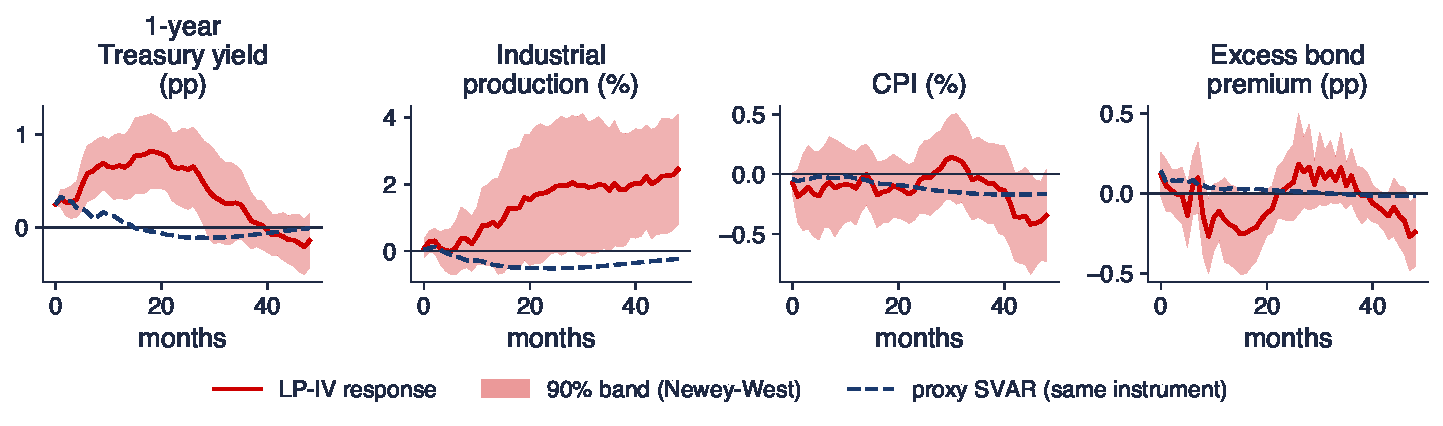
\includegraphics[width=0.97\textwidth,height=0.55\textheight,keepaspectratio]{ats_ch3_lp_gk.pdf}
\end{center}
\vspace{-0.25cm}
\begin{itemize}
    \item LP-IV cu FF4 ca instrument pentru randamentul la 1 an, 2 laguri ale tuturor variabilelor și ale instrumentului drept controale, origini 1990:1--2012:6 ($T = 270$) \refRam; linia întreruptă: proxy SVAR
\end{itemize}
\quantlet{ATS\_ch3\_lp\_vs\_var}{\qlurl{ATS_ch3_lp_vs_var}}
\end{frame}

\begin{frame}{Interpretarea comparației LP-IV cu proxy SVAR}
\itemsize{\small}
\begin{itemize}
    \item Prima etapă la impact: $F = 21{,}5$; după 24 de luni IP: LP-IV 1{,}84\% (SE 1{,}17), proxy SVAR \ensuremath{-}0{,}52\%
    \item IPC după 24 de luni: LP-IV \ensuremath{-}0{,}05\% (SE 0{,}17), proxy SVAR \ensuremath{-}0{,}12\%: benzile LP conțin traiectoria VAR aproape peste tot
    \item LP-IV implică o creștere mult mai persistentă a randamentului: cei doi estimatori răspund la întrebări ușor diferite cînd traiectoria dobînzii diferă
    \begin{itemize}
        \item răspunsul pozitiv al producției în LP, semnalat de \refRam, este imprecis și sensibil la eșantion: nu îl citiți ca o înăsprire expansionistă
    \end{itemize}
\end{itemize}
\end{frame}

\begin{frame}{Proiecții locale dependente de stare (1/2)}
\itemsize{\small}
\begin{itemize}
    \item Interacționăm totul cu indicatorul de stare din perioada anterioară, $I_{t-1}$:
    \begin{itemize}
        \item $y_{t+h} = I_{t-1}[\alpha_{A,h} + \beta_{A,h}x_t + \dots] + (1 - I_{t-1})[\alpha_{B,h} + \beta_{B,h}x_t + \dots] + \xi_{t+h}$
        \item $I_{t-1} = 1$ în starea A (de exemplu subutilizare), 0 în starea B; $\beta_{A,h}$, $\beta_{B,h}$: răspunsurile la orizontul $h$ în fiecare stare; $\alpha$: termeni liberi specifici stării
    \end{itemize}
    \item Ce măsoară LP aici
    \begin{itemize}
        \item starea se poate schimba după șoc: LP măsoară răspunsul mediu dată fiind starea inițială, inclusiv tranzițiile
        \item nu este nevoie să modelăm dinamica stării, spre deosebire de un VAR cu prag sau cu tranziție netedă (\atschlink{https://danpele.github.io/Advanced-Time-Series/RO/Cursuri/capitol2_rupturi_structurale_modele_neliniare.pdf}{Capitolul 2})
    \end{itemize}
\end{itemize}
\end{frame}

\begin{frame}{Proiecții locale dependente de stare (2/2)}
\itemsize{\small}
\begin{itemize}
    \item Studiu de caz \refRZ: sînt multiplicatorii cheltuielilor publice mai mari în perioadele de subutilizare a resurselor?
    \begin{itemize}
        \item date trimestriale SUA 1889--2015; șocul de știri militare (Ramey) scalat la PIB-ul potențial
        \item subutilizare = șomaj $\ge 6{,}5\%$ în $t - 1$ (36\% dintre trimestre)
        \item LP-IV cumulat al producției pe cheltuielile publice, 4 laguri ale știrilor, producției și cheltuielilor, Newey--West cu $h + 1$ laguri
    \end{itemize}
\end{itemize}
\end{frame}

\begin{frame}{Multiplicatorii cheltuielilor publice după starea economiei}
\itemsize{\footnotesize}
\begin{center}
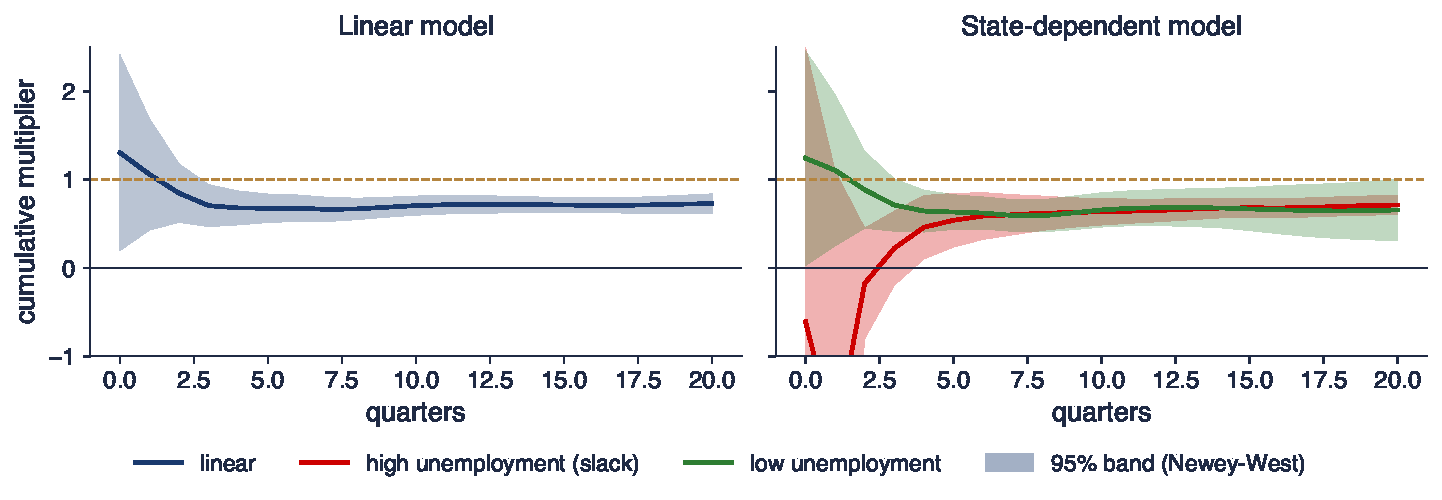
\includegraphics[width=0.97\textwidth,height=0.64\textheight,keepaspectratio]{ats_ch3_rz.pdf}
\end{center}
\vspace{-0.25cm}
\begin{itemize}
    \item Multiplicatorul cumulat $\sum_{j\le h}\Delta y_{t+j}/\sum_{j\le h}\Delta g_{t+j}$ pe orizonturi; benzi Newey--West de 95\%; linia întreruptă: multiplicatorul egal cu unu
\end{itemize}
\quantlet{ATS\_ch3\_state\_dependent\_lp}{\qlurl{ATS_ch3_state_dependent_lp}}
\end{frame}

\begin{frame}{Interpretarea multiplicatorilor dependenți de stare}
\itemsize{\small}
\begin{itemize}
    \item Liniar: 0{,}67 la doi ani (SE 0{,}06) și 0{,}71 la patru ani (SE 0{,}04)
    \item Șomaj ridicat: 0{,}62 și 0{,}68; șomaj scăzut: 0{,}59 și 0{,}66
    \item În acord cu \refRZ: multiplicatori sub unu în ambele stări și nicio diferență semnificativă între ele
    \item Argumentul pentru LP aici: un VAR ar impune aceeași dinamică în ambele stări dacă tranzițiile între stări nu sînt modelate
\end{itemize}
\end{frame}

\begin{frame}{Recapitulare: proiecții locale}
\itemsize{\small}
\begin{itemize}
    \item LP = o regresie pe orizont; inferență HAC sau cu lag augmentation
    \item LP și VAR țintesc aceleași răspunsuri; eșantioanele finite schimbă deplasare pe varianță
    \item LP-IV folosește instrumente externe fără inversabilitate, cu un cost în precizie
    \item Dependența de stare este naturală în LP: RZ găsesc multiplicatori sub unu și în perioade de subutilizare, și în perioade normale
\end{itemize}
\end{frame}


%=============================================================================
\section{România și efectele de propagare din zona euro}
%=============================================================================

\begin{frame}{Politica monetară într-o economie mică și deschisă}
\itemsize{\footnotesize}
\begin{columns}[T]
\begin{column}{0.36\textwidth}
\centering

\includegraphics[height=0.34\textheight]{ch0_bnr_palace_2015.jpg}\\[1mm]
\imgcap{Banca Națională a României, București}
\imgcredit{https://commons.wikimedia.org/wiki/File:Bucharest_-_BNR_Palace_(19644434340).jpg}{Foto: Ștefan Jurcă (2015); CC BY 2.0; Wikimedia Commons}
\end{column}
\begin{column}{0.62\textwidth}
\begin{itemize}
    \item BNR țintește inflația din august 2005 (ținta 2,5\% $\pm$ 1 pp din 2013), în regim de managed float al leului
    \begin{itemize}
        \item dobînda interbancară ROBOR 3M transmite dobînda de politică monetară și condițiile de lichiditate; o folosim ca indicator de politică
    \end{itemize}
    \item Probleme de identificare specifice României
    \begin{itemize}
        \item eșantion scurt (20 de ani), schimbări structurale (2008--2009, 2020, 2022), prețuri administrate și modificări de accize
        \item șocurile externe domină: zona euro preia majoritatea exporturilor românești; politica BCE mișcă dobînzile românești și leul
    \end{itemize}
    \item Abordarea noastră: un VAR recursiv transparent, cu zona euro pe primul loc, apoi un șoc extern BCE cu LP
\end{itemize}
\end{column}
\end{columns}
\end{frame}

\begin{frame}{Date pentru România și zona euro}
\itemsize{\footnotesize}
\begin{center}
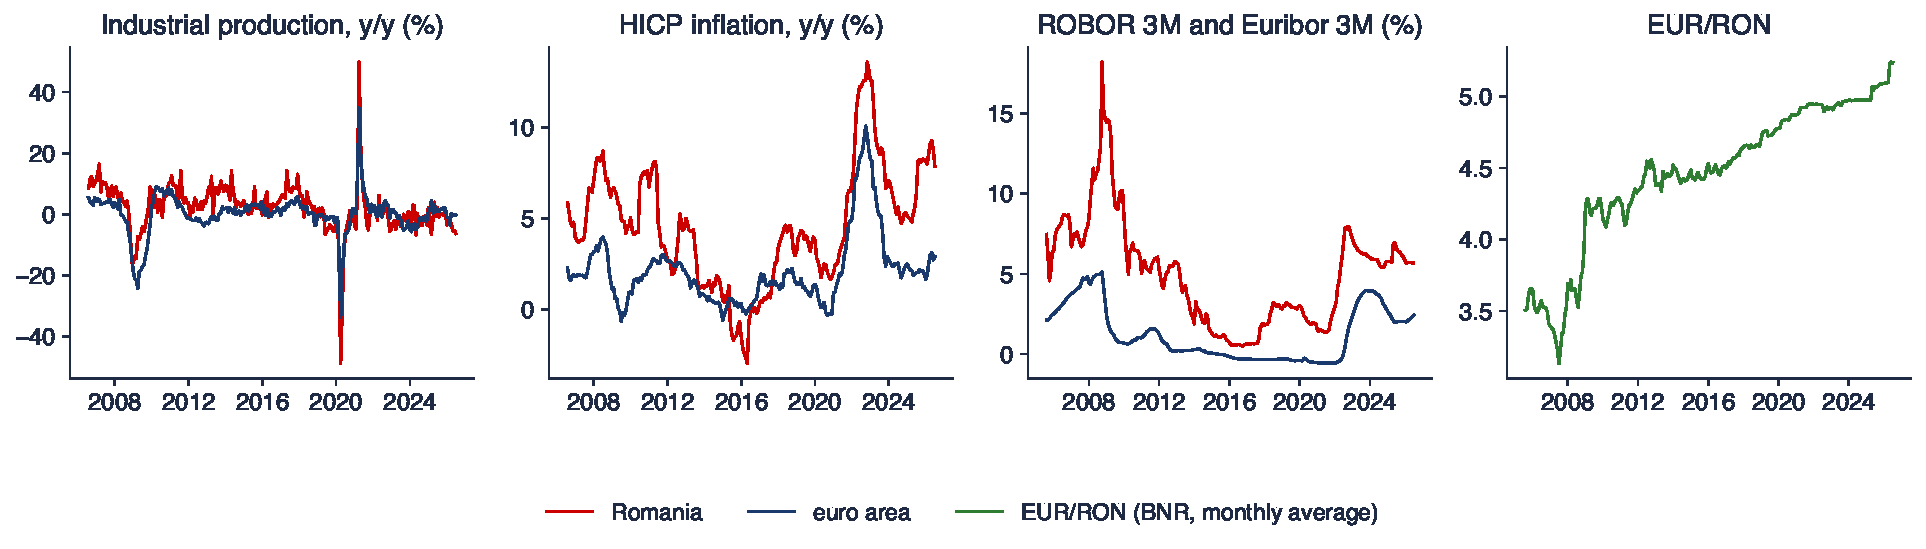
\includegraphics[width=0.97\textwidth,height=0.53\textheight,keepaspectratio]{ats_ch3_ro_data.pdf}
\end{center}
\vspace{-0.25cm}
\begin{itemize}
    \item Lunar, august 2005--iulie 2026: IP (ajustată sezonier), IAPC, dobînzile pieței monetare la 3 luni (Eurostat), EUR/RON (cursul de referință BNR, media lunară)
\end{itemize}
\quantlet{ATS\_ch3\_romania}{\qlurl{ATS_ch3_romania}}
\end{frame}

\begin{frame}{Interpretarea datelor pentru România}
\itemsize{\small}
\begin{itemize}
    \item Inflația IAPC a atins maximul de 13{,}6\% în noiembrie 2022 și este 7{,}9\% în ultima lună; ROBOR 3M a ajuns la 18{,}2\% în criza de lichiditate din 2008
    \item EUR/RON a crescut de la 3{,}51 la 5{,}24: o depreciere tendențială cu perioade lungi de stabilitate, sub regimul de managed float
    \item IP din România și din zona euro evoluează împreună, inclusiv prăbușirea din 2020: un argument puternic pentru un bloc extern
    \item Valorile extreme (2008, 2020, 2022) vor domina estimațiile unui VAR mic: verificați robustețea fără ele
\end{itemize}
\end{frame}

\begin{frame}{Un VAR pentru România cu un bloc al zonei euro}
\itemsize{\small}
\begin{itemize}
    \item $y_t$ = (IP ZE, IAPC ZE, Euribor 3M, IP RO, IAPC RO, ROBOR 3M, EUR/RON), logaritmi $\times 100$ cu excepția dobînzilor; termen liber și variabile dummy lunare (IAPC nu este ajustat sezonier)
    \begin{itemize}
        \item numărul de laguri: BIC și HQ aleg 2, AIC 6; folosim 2 ($T = 250$); cea mai mare rădăcină 1{,}006: niveluri, rădăcină aproape unitară, fără corecția deplasării
    \end{itemize}
    \item Identificarea (Cholesky, în această ordine): zona euro nu reacționează la România în aceeași lună; ROBOR reacționează în aceeași lună la activitatea și prețurile din România; cursul de schimb reacționează la toate
    \begin{itemize}
        \item restricția zero pentru zona euro este credibilă (România este mică); poziția ROBOR înaintea EUR/RON este discutabilă
        \item un VAR cu exogenitate pe blocuri ar anula și efectele cu lag ale României asupra zonei euro (Seminarul 3, B2 discută ordonările)
    \end{itemize}
\end{itemize}
\end{frame}

\begin{frame}{Răspunsuri la un șoc al dobînzii interne și la unul al zonei euro}
\itemsize{\footnotesize}
\begin{center}
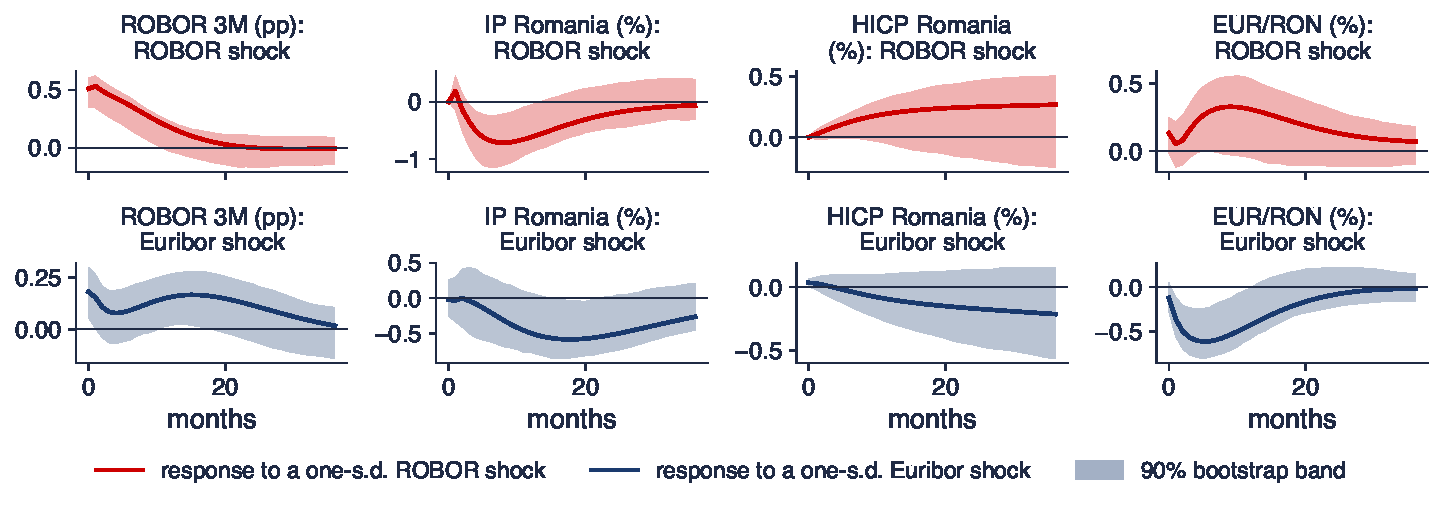
\includegraphics[width=0.97\textwidth,height=0.65\textheight,keepaspectratio]{ats_ch3_ro_var.pdf}
\end{center}
\vspace{-0.25cm}
\begin{itemize}
    \item VAR(2), Cholesky cu blocul zonei euro pe primul loc; șocuri de o abatere standard (ROBOR 0{,}51 pp, Euribor 0{,}09 pp); benzi bootstrap de 90\%
\end{itemize}
\quantlet{ATS\_ch3\_romania}{\qlurl{ATS_ch3_romania}}
\end{frame}

\begin{frame}{Interpretarea răspunsurilor pentru România}
\itemsize{\small}
\begin{itemize}
    \item Șocul ROBOR: IP \ensuremath{-}0{,}62\% după 12 luni (banda [\ensuremath{-}0{,}88; \ensuremath{-}0{,}06]); IAPC 0{,}20\% (banda [\ensuremath{-}0{,}06; 0{,}34]); EUR/RON 0{,}31\%
    \begin{itemize}
        \item o anomalie a prețurilor și una a cursului de schimb (depreciere după o înăsprire): inovația ROBOR conține încă reacția BNR la inflație și la presiunea asupra leului
    \end{itemize}
    \item Șocul Euribor: IP din România \ensuremath{-}0{,}50\% după 12 luni (banda [\ensuremath{-}0{,}77; 0{,}07]); IAPC \ensuremath{-}0{,}10\%; ROBOR 0{,}16 pp
    \item Pe scurt: VAR-ul recursiv identifică credibil blocul zonei euro și slab șocul de politică internă
\end{itemize}
\end{frame}

\begin{frame}{Contribuția zonei euro la fluctuațiile din România}
\itemsize{\small}
\begin{center}
\scriptsize
\begin{tabular}{lrrrr}
\toprule
\textbf{Variabila} & \textbf{șocuri ZE, 12 luni} & \textbf{șocuri ZE, 36 de luni} & \textbf{șoc ROBOR, 12 luni} & \textbf{șoc propriu, 12 luni} \\
\midrule
IP România & 46\% & 37\% & 8\% & 41\% \\
IAPC România & 44\% & 55\% & 3\% & 42\% \\
ROBOR 3M & 30\% & 39\% & 59\% & -- \\
EUR/RON & 25\% & 23\% & 6\% & 58\% \\
\bottomrule
\end{tabular}
\end{center}
\begin{itemize}
    \item Descompunerea varianței erorii de prognoză din VAR(2) recursiv; șocuri ZE = cele trei șocuri ale zonei euro împreună
    \item Șocurile zonei euro explică 46\% din IP din România la un an și 55\% din IAPC la trei ani; șocul dobînzii interne explică mai puțin de o zecime din fiecare
    \item Ponderile sînt la fel de credibile ca ordonarea; cu un VAR cu exogenitate pe blocuri ele sînt o limită inferioară a influenței externe
\end{itemize}
\end{frame}

\begin{frame}{Șocuri de politică BCE și România: proiecții locale}
\itemsize{\footnotesize}
\begin{center}
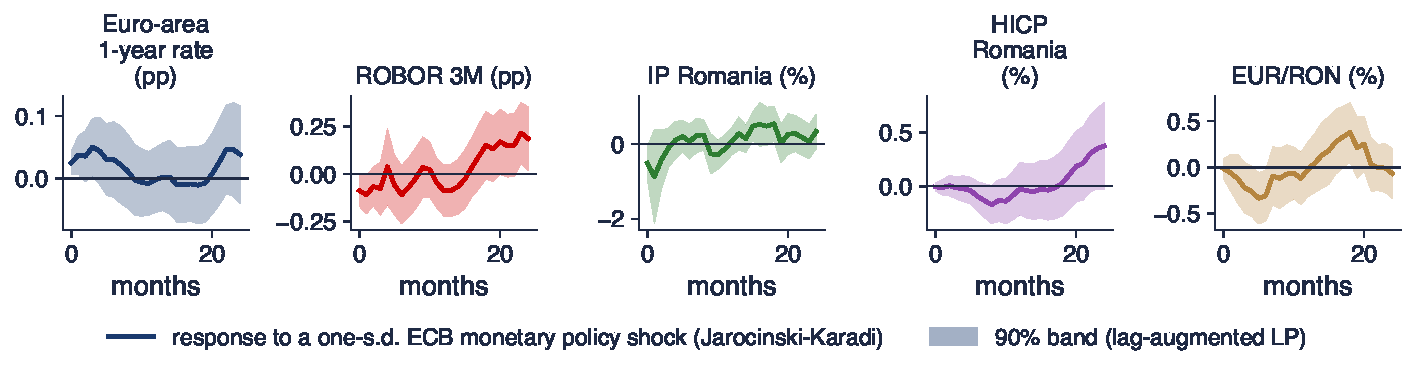
\includegraphics[width=0.97\textwidth,height=0.48\textheight,keepaspectratio]{ats_ch3_ro_lp.pdf}
\end{center}
\vspace{-0.25cm}
\begin{itemize}
    \item Șocul: șocul pur de politică monetară din \refJK\ (actualizarea autorilor, o abatere standard = 3{,}2 bp); 3 laguri ale tuturor variabilelor și ale șocului (lag augmentation), variabile dummy lunare; origini 2005:8--2025:10
\end{itemize}
\quantlet{ATS\_ch3\_romania}{\qlurl{ATS_ch3_romania}}
\end{frame}

\begin{frame}{Interpretarea proiecțiilor de propagare}
\itemsize{\small}
\begin{itemize}
    \item Întîi relevanța: dobînda la 1 an din zona euro crește cu 0{,}03 pp la impact (SE 0{,}01); statistica $F$ din prima etapă $= 4{,}8$ (impact) și 4{,}0 (o lună)
    \begin{itemize}
        \item mediile lunare diluează o surpriză din ziua anunțului: șocul este un instrument slab pentru dobînzile lunare din zona euro
    \end{itemize}
    \item IAPC din România: \ensuremath{-}0{,}02\% după 12 luni (SE 0{,}15), 0{,}37\% după 24 (SE 0{,}25); EUR/RON \ensuremath{-}0{,}31\% după 6 luni (SE 0{,}17)
    \item Concluzia prudentă: cu un șoc extern slab și 20 de ani de date, efectele de propagare asupra prețurilor din România nu sînt determinate; o mulțime robustă la instrumente slabe este largă (Seminarul 3, C1)
\end{itemize}
\end{frame}

\begin{frame}{Concluzii pentru România}
\itemsize{\small}
\begin{itemize}
    \item Rezultate robuste
    \begin{itemize}
        \item șocurile din zona euro explică o parte mare din fluctuațiile producției și ale prețurilor din România
        \item o înăsprire în zona euro scade IP din România în decurs de un an în VAR-ul recursiv
    \end{itemize}
    \item Rezultate fragile
    \begin{itemize}
        \item efectul unui șoc ROBOR intern asupra prețurilor și leului: anomaliile semnalează un eșec al identificării, nu un fapt despre România
        \item mărimea efectelor politicii BCE asupra inflației din România: instrumentul este slab la frecvență lunară
    \end{itemize}
    \item Pașii următori (proiecte)
    \begin{itemize}
        \item surprize la ședințele de politică monetară ale BNR, din cotațiile ROBOR sau FRA în jurul anunțurilor, folosite ca proxy
        \item restricții de semn (o înăsprire apreciază leul și scade prețurile) și un VAR bayesian cu shrinkage (\atschlink{https://danpele.github.io/Advanced-Time-Series/RO/Cursuri/capitol5_bvar_modele_factoriale_nowcasting.pdf}{Capitolul 5})
    \end{itemize}
\end{itemize}
\end{frame}

\begin{frame}{Recapitulare: efectele de propagare din zona euro asupra României}
\itemsize{\small}
\begin{itemize}
    \item Puneți vecinul mare pe primul loc: blocul zonei euro este credibil exogen în aceeași lună
    \item Un șoc ROBOR recursiv produce anomalii ale prețurilor și ale cursului de schimb
    \item Șocurile externe BCE sînt instrumente slabe la frecvență lunară: raportați incertitudinea, nu o ascundeți
\end{itemize}
\end{frame}


%=============================================================================
\section{AI în descoperirea științifică}
%=============================================================================

\begin{frame}{O întrebare deschisă}
\itemsize{\small}
\begin{itemize}
    \item Cît de puternic se transmite politica monetară a BCE asupra inflației din România și s-a schimbat această transmisie după 2022?
    \begin{itemize}
        \item formal: $H_0$: $\theta_{12} = 0$, răspunsul IAPC din România după 12 luni la un șoc de 25 bp al dobînzii din zona euro, testat cu o mulțime Anderson--Rubin valabilă și pentru instrumente slabe
        \item infirmată de o mulțime de 90\% mărginită care exclude zero, pentru un șoc, un orizont și un eșantion preînregistrate
    \end{itemize}
    \item De ce contează: România pregătește aderarea la zona euro; BNR trebuie să știe cîtă inflație este importată
    \begin{itemize}
        \item literatura de pornire: \refJK, \refSWc, \refMSW, \refPW, \refLPW
    \end{itemize}
\end{itemize}
\end{frame}

\begin{frame}{Bucla de cercetare cu un asistent AI}
\itemsize{\footnotesize}
\begin{itemize}
    \item Un asistent AI (un LLM precum Claude, ChatGPT, Gemini sau Copilot) accelerează fiecare etapă; Semantic Scholar și Elicit ajută la literatură
    \begin{itemize}
        \item \textbf{literatura}: \aiprompt{Listează articole recenzate care estimează efectele de propagare ale politicii monetare din zona euro asupra României sau a Europei Centrale și de Est cu șocuri de frecvență înaltă; dă DOI-urile.} Apoi verificați fiecare DOI pe Crossref
        \item \textbf{ipoteza}: \aiprompt{Propune trei canale (comerț, curs de schimb, finanțarea băncilor) și cîte o implicație observabilă pentru fiecare.}
        \item \textbf{cod și replicare}: cereți o funcție LP-IV, apoi reproduceți întîi o cifră cunoscută (statistica $F$ din prima etapă din acest curs)
        \item \textbf{robustețe și critică}: \aiprompt{Joacă rolul unui recenzent ostil: enumeră toate felurile în care această identificare a efectelor BCE ar putea eșua.}
    \end{itemize}
    \item Raportul: ce s-a cerut, ce s-a păstrat, ce s-a respins (AI\_USE.md, AI\_ERRORS.md)
\end{itemize}
\end{frame}

\begin{frame}{Verificări necesare}
\itemsize{\small}
\begin{itemize}
    \item Fiecare referință există și spune ce se afirmă (DOI-ul funcționează, titlul coincide, rezultatul se află în lucrare)
    \item Șocul este datat corect: surprizele din zilele anunțurilor se adună în interiorul lunii, nu se mută niciodată înainte
    \item Relevanța se raportează (statistica $F$ din prima etapă cu varianță HAC) înainte de interpretarea oricărui răspuns
    \item Lagurile, orizonturile, eșantionul și tratarea anului 2020 sînt fixate înaintea rezultatelor; toate variantele sînt raportate
    \item Un rezumat AI despre un „efect de propagare semnificativ” se verifică pe mulțimea de încredere, nu pe estimația punctuală
\end{itemize}
\end{frame}

\begin{frame}{Mini-studiu de caz: robustețea unei singure cifre}
\itemsize{\footnotesize}
\begin{center}
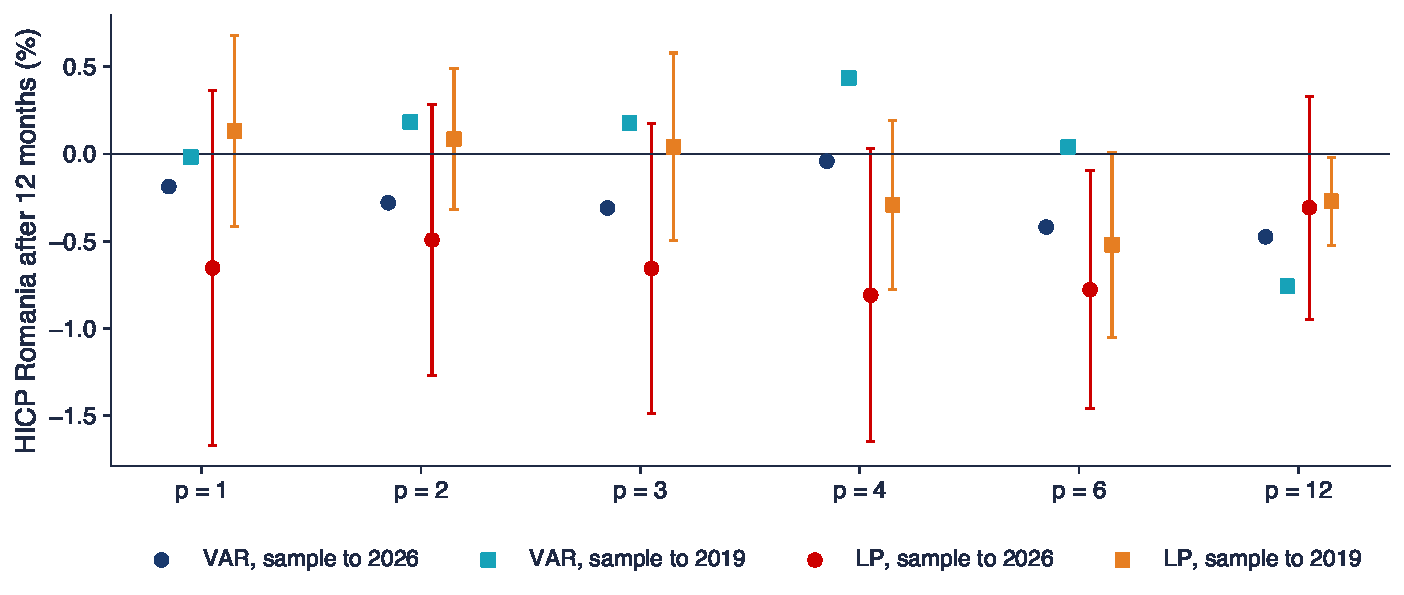
\includegraphics[width=0.97\textwidth,height=0.55\textheight,keepaspectratio]{ats_ch3_ai_case.pdf}
\end{center}
\vspace{-0.25cm}
\begin{itemize}
    \item Răspunsul IAPC din România după 12 luni la un șoc Euribor de 25 bp: VAR recursiv și LP recursivă (bare Newey--West de 90\%), numărul de laguri $p$, eșantioane care se încheie în 2019 și în 2026
    \item Cele 24 de estimații variază între \ensuremath{-}0{,}81\% și 0{,}44\%, iar 7 dintre ele sînt pozitive: semnul depinde de numărul de laguri și de datele de după 2020; un asistent AI care raportează una dintre ele „cu încredere” greșește
\end{itemize}
\quantlet{ATS\_ch3\_romania}{\qlurl{ATS_ch3_romania}}
\end{frame}

\begin{frame}{Idee de proiect}
\itemsize{\small}
\begin{itemize}
    \item \textbf{Efectele politicii monetare din zona euro asupra României}: întîi replicare, apoi extindere
    \begin{itemize}
        \item replicați: modelul proxy SVAR din \refGK\ (în acest curs: $F = 17{,}7$, saltul primei de risc) și LP pentru România din acest curs
        \item extindeți: surprizele zilnice BCE agregate lunar cu metoda de mediere Gertler--Karadi; o versiune trimestrială cu PIB; mulțimi Anderson--Rubin; restricții de semn pe surprize (\refJK)
        \item preînregistrați: șocul, variabilele de rezultat, orizonturile 0--24, regula pentru laguri, tratarea anului 2020 și corecția Holm pentru mai multe variabile
    \end{itemize}
    \item Livrabilele urmează regulile cursului: repository, raport, AI\_USE.md, AI\_ERRORS.md, susținere orală
\end{itemize}
\end{frame}


%=============================================================================
\section{Încheiere}
%=============================================================================

\begin{frame}{Idei de reținut}
\itemsize{\small}
\begin{itemize}
    \item Un VAR structural este o formă redusă plus o ipoteză de identificare; ipoteza este partea economică
    \item Zerourile (pe termen scurt sau lung), semnele, restricțiile narative, heteroscedasticitatea și instrumentele obțin fiecare identificarea pe baza unei alte ipoteze
    \item Identificarea pe mulțimi nu promite mai mult decît dau datele: raportați mulțimea și rolul distribuției a priori
    \item Inferența: bootstrap potrivit cazului, corecția deplasării, benzi simultane, mulțimi robuste la instrumente slabe
    \item LP și VAR estimează aceleași răspunsuri; alegeți după deplasare și varianță și folosiți LP pentru dependența de stare
\end{itemize}
\end{frame}

\begin{frame}{Autoevaluare}
\itemsize{\small}
\begin{columns}[T]
\begin{column}{0.56\textwidth}
\begin{block}{Întrebări}
\begin{itemize}
    \item Cîte restricții identifică exact un SVAR cu cinci variabile?
    \item De ce identifică $\E u_tz_t$ coloana de impact a unui proxy SVAR?
    \item Ce nu reprezintă mediana a posteriori a unui răspuns identificat prin semne?
    \item Cînd bate un VAR proiecțiile locale în eroarea medie pătratică?
    \item De ce nu este valid bootstrap-ul wild pentru un proxy SVAR?
\end{itemize}
\end{block}
\end{column}
\begin{column}{0.40\textwidth}
\begin{block}{Urmează: \atschlink{https://danpele.github.io/Advanced-Time-Series/RO/Cursuri/capitol4_cointegrare_vecm_ardl_panel.pdf}{Capitolul 4}}
\begin{itemize}
    \item Cointegrare: VECM, ARDL și date panel
    \item Restricțiile de termen lung devin restricții asupra vectorilor de cointegrare și asupra trendurilor comune
\end{itemize}
\end{block}
\end{column}
\end{columns}
\end{frame}


%=============================================================================
\section{Anexă}
%=============================================================================

\begin{frame}{Anexă: restricția de termen lung în formă închisă}
\hypertarget{atsapp1}{}\atsappback{atssrc1}{Înapoi}
\itemsize{\small}
\begin{itemize}
    \item VAR stabil: $\sum_{h\ge0}\Phi_h = A(1)^{-1}$, deci matricea răspunsurilor de termen lung este $\Theta(1) = A(1)^{-1}B_0$
    \item $\Theta(1)\Theta(1)' = A(1)^{-1}B_0B_0'A(1)^{-1\prime} = A(1)^{-1}\Sigma_uA(1)^{-1\prime}$, cunoscută din forma redusă
    \item $[\Theta(1)]_{12} = 0$ face $\Theta(1)$ inferior triunghiulară: $\Theta(1) = \mathrm{chol}(A(1)^{-1}\Sigma_uA(1)^{-1\prime})$, unică pentru o diagonală pozitivă
    \item Deci $B_0 = A(1)\Theta(1)$; verificăm $B_0B_0' = \Sigma_u$; semnele se normalizează apoi (oferta crește producția pe termen lung)
\end{itemize}
\end{frame}

\begin{frame}{Anexă: identificarea coloanei $b_1$ prin proxy}
\hypertarget{atsapp2}{}\atsappback{atssrc2}{Înapoi}
\itemsize{\small}
\begin{itemize}
    \item $u_t = B_0\varepsilon_t = b_1\varepsilon_{1t} + \sum_{j\ge2}b_j\varepsilon_{jt}$
    \item $\E u_tz_t = b_1\E\varepsilon_{1t}z_t + \sum_{j\ge2}b_j\E\varepsilon_{jt}z_t = \alpha b_1$ din exogenitate
    \item Impacturile relative $b_{i1}/b_{11} = \E u_{it}z_t/\E u_{1t}z_t$ cer $\alpha \ne 0$ (relevanța); scala lui $b_1$ rezultă din $b_1'\Sigma_u^{-1}b_1 = 1$
\end{itemize}
\end{frame}

\begin{frame}{Anexă: LP și VAR coincid pînă la orizontul $p$}
\hypertarget{atsapp3}{}\atsappback{atssrc3}{Înapoi}
\itemsize{\small}
\begin{itemize}
    \item Fie $w_t = (y_{t-1}, \dots, y_{t-p})$, iar șocul inovația $\tilde x_t = x_t - \mathrm{proj}(x_t\mid w_t)$
    \item Coeficientul LP: $\beta_h = \Cov(y_{t+h}, \tilde x_t)/\Var(\tilde x_t)$ (Frisch--Waugh)
    \item VAR($p$) reproduce exact autocovarianțele $\Gamma_0, \dots, \Gamma_p$; pentru $h \le p$, $\Cov(y_{t+h}, \tilde x_t)$ depinde doar de ele, deci ambele dau același $\beta_h$ \refPW
    \item Pentru $h > p$, VAR-ul își extrapolează propriile autocovarianțe: sursa deplasării unui VAR scurt și a varianței mai mici
\end{itemize}
\end{frame}


%=============================================================================
\section{Bibliografie}
%=============================================================================

\begin{frame}{Bibliografie (1/4)}
\itemsize{\tiny}
\begin{itemize}
    \item Antolín-Díaz, J., \& Rubio-Ramírez, J. F. (2018). Narrative sign restrictions for SVARs. \textit{American Economic Review}, 108(10), 2802--2829. \href{https://doi.org/10.1257/aer.20161852}{doi:10.1257/aer.20161852}
    \item Arias, J. E., Rubio-Ramírez, J. F., \& Waggoner, D. F. (2018). Inference based on structural vector autoregressions identified with sign and zero restrictions: Theory and applications. \textit{Econometrica}, 86(2), 685--720. \href{https://doi.org/10.3982/ECTA14468}{doi:10.3982/ECTA14468}
    \item Bauer, M. D., \& Swanson, E. T. (2023). A reassessment of monetary policy surprises and high-frequency identification. \textit{NBER Macroeconomics Annual}, 37, 87--155. \href{https://doi.org/10.1086/723574}{doi:10.1086/723574}
    \item Baumeister, C., \& Hamilton, J. D. (2015). Sign restrictions, structural vector autoregressions, and useful prior information. \textit{Econometrica}, 83(5), 1963--1999. \href{https://doi.org/10.3982/ECTA12356}{doi:10.3982/ECTA12356}
    \item Baumeister, C., \& Hamilton, J. D. (2019). Structural interpretation of vector autoregressions with incomplete identification: Revisiting the role of oil supply and demand shocks. \textit{American Economic Review}, 109(5), 1873--1910. \href{https://doi.org/10.1257/aer.20151569}{doi:10.1257/aer.20151569}
    \item Blanchard, O. J., \& Quah, D. (1989). The dynamic effects of aggregate demand and supply disturbances. \textit{American Economic Review}, 79(4), 655--673. \href{https://www.jstor.org/stable/1827924}{jstor.org}
    \item Blanchard, O., \& Perotti, R. (2002). An empirical characterization of the dynamic effects of changes in government spending and taxes on output. \textit{The Quarterly Journal of Economics}, 117(4), 1329--1368. \href{https://doi.org/10.1162/003355302320935043}{doi:10.1162/003355302320935043}
    \item Christiano, L. J., Eichenbaum, M., \& Evans, C. L. (1999). Monetary policy shocks: What have we learned and to what end? In J. B. Taylor \& M. Woodford (Eds.), \textit{Handbook of Macroeconomics} (Vol.\ 1A, pp.\ 65--148). Elsevier. \href{https://doi.org/10.1016/S1574-0048(99)01005-8}{doi:10.1016/S1574-0048(99)01005-8}
    \item Faust, J., \& Leeper, E. M. (1997). When do long-run identifying restrictions give reliable results? \textit{Journal of Business \& Economic Statistics}, 15(3), 345--353. \href{https://doi.org/10.1080/07350015.1997.10524712}{doi:10.1080/07350015.1997.10524712}
    \item Fry, R., \& Pagan, A. (2011). Sign restrictions in structural vector autoregressions: A critical review. \textit{Journal of Economic Literature}, 49(4), 938--960. \href{https://doi.org/10.1257/jel.49.4.938}{doi:10.1257/jel.49.4.938}
    \item Galí, J. (1999). Technology, employment, and the business cycle: Do technology shocks explain aggregate fluctuations? \textit{American Economic Review}, 89(1), 249--271. \href{https://doi.org/10.1257/aer.89.1.249}{doi:10.1257/aer.89.1.249}
\end{itemize}
\end{frame}

\begin{frame}{Bibliografie (2/4)}
\itemsize{\tiny}
\begin{itemize}
    \item Gertler, M., \& Karadi, P. (2015). Monetary policy surprises, credit costs, and economic activity. \textit{American Economic Journal: Macroeconomics}, 7(1), 44--76. \href{https://doi.org/10.1257/mac.20130329}{doi:10.1257/mac.20130329}
    \item Giacomini, R., \& Kitagawa, T. (2021). Robust Bayesian inference for set-identified models. \textit{Econometrica}, 89(4), 1519--1556. \href{https://doi.org/10.3982/ecta16773}{doi:10.3982/ecta16773}
    \item Gilchrist, S., \& Zakrajšek, E. (2012). Credit spreads and business cycle fluctuations. \textit{American Economic Review}, 102(4), 1692--1720. \href{https://doi.org/10.1257/aer.102.4.1692}{doi:10.1257/aer.102.4.1692}
    \item Gonçalves, S., \& Kilian, L. (2004). Bootstrapping autoregressions with conditional heteroskedasticity of unknown form. \textit{Journal of Econometrics}, 123(1), 89--120. \href{https://doi.org/10.1016/j.jeconom.2003.10.030}{doi:10.1016/j.jeconom.2003.10.030}
    \item Gürkaynak, R. S., Sack, B., \& Swanson, E. T. (2005). Do actions speak louder than words? The response of asset prices to monetary policy actions and statements. \textit{International Journal of Central Banking}, 1(1), 55--93. \href{https://www.ijcb.org/journal/ijcb05q2a2.htm}{ijcb.org}
    \item Hamilton, J. D. (1994). \textit{Time Series Analysis}. Princeton University Press. \href{https://doi.org/10.2307/j.ctv14jx6sm}{doi:10.2307/j.ctv14jx6sm}
    \item Jarociński, M., \& Karadi, P. (2020). Deconstructing monetary policy surprises: The role of information shocks. \textit{American Economic Journal: Macroeconomics}, 12(2), 1--43. \href{https://doi.org/10.1257/mac.20180090}{doi:10.1257/mac.20180090}
    \item Jentsch, C., \& Lunsford, K. G. (2019). The dynamic effects of personal and corporate income tax changes in the United States: Comment. \textit{American Economic Review}, 109(7), 2655--2678. \href{https://doi.org/10.1257/aer.20162011}{doi:10.1257/aer.20162011}
    \item Jordà, Ò. (2005). Estimation and inference of impulse responses by local projections. \textit{American Economic Review}, 95(1), 161--182. \href{https://doi.org/10.1257/0002828053828518}{doi:10.1257/0002828053828518}
    \item Kilian, L., \& Lütkepohl, H. (2017). \textit{Structural Vector Autoregressive Analysis}. Cambridge University Press. \href{https://doi.org/10.1017/9781108164818}{doi:10.1017/9781108164818}
    \item Kilian, L. (2019). Measuring global real economic activity: Do recent critiques hold up to scrutiny? \textit{Economics Letters}, 178, 106--110. \href{https://doi.org/10.1016/j.econlet.2019.03.001}{doi:10.1016/j.econlet.2019.03.001}
\end{itemize}
\end{frame}

\begin{frame}{Bibliografie (3/4)}
\itemsize{\tiny}
\begin{itemize}
    \item Kilian, L. (2009). Not all oil price shocks are alike: Disentangling demand and supply shocks in the crude oil market. \textit{American Economic Review}, 99(3), 1053--1069. \href{https://doi.org/10.1257/aer.99.3.1053}{doi:10.1257/aer.99.3.1053}
    \item Kilian, L. (1998). Small-sample confidence intervals for impulse response functions. \textit{The Review of Economics and Statistics}, 80(2), 218--230. \href{https://doi.org/10.1162/003465398557465}{doi:10.1162/003465398557465}
    \item Kuttner, K. N. (2001). Monetary policy surprises and interest rates: Evidence from the Fed funds futures market. \textit{Journal of Monetary Economics}, 47(3), 523--544. \href{https://doi.org/10.1016/S0304-3932(01)00055-1}{doi:10.1016/S0304-3932(01)00055-1}
    \item Lanne, M., \& Lütkepohl, H. (2008). Identifying monetary policy shocks via changes in volatility. \textit{Journal of Money, Credit and Banking}, 40(6), 1131--1149. \href{https://doi.org/10.1111/j.1538-4616.2008.00151.x}{doi:10.1111/j.1538-4616.2008.00151.x}
    \item Li, D., Plagborg-Møller, M., \& Wolf, C. K. (2024). Local projections vs.\ VARs: Lessons from thousands of DGPs. \textit{Journal of Econometrics}, 244(2), 105722. \href{https://doi.org/10.1016/j.jeconom.2024.105722}{doi:10.1016/j.jeconom.2024.105722}
    \item Lütkepohl, H. (2005). \textit{New Introduction to Multiple Time Series Analysis}. Springer. \href{https://doi.org/10.1007/978-3-540-27752-1}{doi:10.1007/978-3-540-27752-1}
    \item Mertens, K., \& Ravn, M. O. (2013). The dynamic effects of personal and corporate income tax changes in the United States. \textit{American Economic Review}, 103(4), 1212--1247. \href{https://doi.org/10.1257/aer.103.4.1212}{doi:10.1257/aer.103.4.1212}
    \item Montiel Olea, J. L., \& Plagborg-Møller, M. (2021). Local projection inference is simpler and more robust than you think. \textit{Econometrica}, 89(4), 1789--1823. \href{https://doi.org/10.3982/ECTA18756}{doi:10.3982/ECTA18756}
    \item Montiel Olea, J. L., \& Plagborg-Møller, M. (2019). Simultaneous confidence bands: Theory, implementation, and an application to SVARs. \textit{Journal of Applied Econometrics}, 34(1), 1--17. \href{https://doi.org/10.1002/jae.2656}{doi:10.1002/jae.2656}
    \item Montiel Olea, J. L., Stock, J. H., \& Watson, M. W. (2021). Inference in structural vector autoregressions identified with an external instrument. \textit{Journal of Econometrics}, 225(1), 74--87. \href{https://doi.org/10.1016/j.jeconom.2020.05.014}{doi:10.1016/j.jeconom.2020.05.014}
    \item Nakamura, E., \& Steinsson, J. (2018). High-frequency identification of monetary non-neutrality: The information effect. \textit{The Quarterly Journal of Economics}, 133(3), 1283--1330. \href{https://doi.org/10.1093/qje/qjy004}{doi:10.1093/qje/qjy004}
\end{itemize}
\end{frame}

\begin{frame}{Bibliografie (4/4)}
\itemsize{\tiny}
\begin{itemize}
    \item Plagborg-Møller, M., \& Wolf, C. K. (2021). Local projections and VARs estimate the same impulse responses. \textit{Econometrica}, 89(2), 955--980. \href{https://doi.org/10.3982/ECTA17813}{doi:10.3982/ECTA17813}
    \item Ramey, V. A. (2016). Macroeconomic shocks and their propagation. In J. B. Taylor \& H. Uhlig (Eds.), \textit{Handbook of Macroeconomics} (Vol.\ 2A, pp.\ 71--162). Elsevier. \href{https://doi.org/10.1016/bs.hesmac.2016.03.003}{doi:10.1016/bs.hesmac.2016.03.003}
    \item Ramey, V. A., \& Zubairy, S. (2018). Government spending multipliers in good times and in bad: Evidence from US historical data. \textit{Journal of Political Economy}, 126(2), 850--901. \href{https://doi.org/10.1086/696277}{doi:10.1086/696277}
    \item Rigobon, R. (2003). Identification through heteroskedasticity. \textit{The Review of Economics and Statistics}, 85(4), 777--792. \href{https://doi.org/10.1162/003465303772815727}{doi:10.1162/003465303772815727}
    \item Romer, C. D., \& Romer, D. H. (2004). A new measure of monetary shocks: Derivation and implications. \textit{American Economic Review}, 94(4), 1055--1084. \href{https://doi.org/10.1257/0002828042002651}{doi:10.1257/0002828042002651}
    \item Rubio-Ramírez, J. F., Waggoner, D. F., \& Zha, T. (2010). Structural vector autoregressions: Theory of identification and algorithms for inference. \textit{The Review of Economic Studies}, 77(2), 665--696. \href{https://doi.org/10.1111/j.1467-937X.2009.00578.x}{doi:10.1111/j.1467-937X.2009.00578.x}
    \item Sims, C. A. (1980). Macroeconomics and reality. \textit{Econometrica}, 48(1), 1--48. \href{https://doi.org/10.2307/1912017}{doi:10.2307/1912017}
    \item Stock, J. H., \& Watson, M. W. (2012). Disentangling the channels of the 2007--09 recession. \textit{Brookings Papers on Economic Activity}, 2012(1), 81--135. \href{https://doi.org/10.1353/eca.2012.0005}{doi:10.1353/eca.2012.0005}
    \item Stock, J. H., \& Watson, M. W. (2018). Identification and estimation of dynamic causal effects in macroeconomics using external instruments. \textit{The Economic Journal}, 128(610), 917--948. \href{https://doi.org/10.1111/ecoj.12593}{doi:10.1111/ecoj.12593}
    \item Stock, J. H., \& Watson, M. W. (2001). Vector autoregressions. \textit{Journal of Economic Perspectives}, 15(4), 101--115. \href{https://doi.org/10.1257/jep.15.4.101}{doi:10.1257/jep.15.4.101}
    \item Uhlig, H. (2005). What are the effects of monetary policy on output? Results from an agnostic identification procedure. \textit{Journal of Monetary Economics}, 52(2), 381--419. \href{https://doi.org/10.1016/j.jmoneco.2004.05.007}{doi:10.1016/j.jmoneco.2004.05.007}
\end{itemize}
\end{frame}

\end{document}
